\documentclass[10pt, oneside]{article}
\usepackage{amsmath, amsthm, amssymb, mathrsfs, wasysym, verbatim, bbm, color, graphicx, geometry, authblk}
\usepackage{booktabs, multirow, makecell,colortbl}
\usepackage{setspace}
%\usepackage{ctex}
%\usepackage{calrsfs}
\usepackage{braket}
\usepackage{caption}
\usepackage{subcaption}
\usepackage{hyperref}
\usepackage{framed}
\usepackage{bm}
\usepackage{tikz}
%\usepackage{mathptmx}
\hypersetup{
	colorlinks=true,
	linkcolor=blue,
	filecolor=blue,      
	urlcolor=blue,
	citecolor=blue,
}

\usetikzlibrary{shapes.geometric, arrows}
% Styles
\tikzstyle{startstop} = [ellipse, minimum width=3cm, minimum height=1cm,
                         text centered, draw=black, fill=red!30]
\tikzstyle{process}   = [rectangle, draw=black, fill=green!20,
                         minimum width=5cm, minimum height=1cm, text centered]
\tikzstyle{decision}  = [diamond, draw=black, fill=yellow!30,
                         aspect=2, text centered, inner sep=1pt]
\tikzstyle{arrow}     = [thick,->,>=stealth]

\geometry{tmargin=0.75in, bmargin=.75in, lmargin=.75in, rmargin=.75in}
\setlength{\parindent}{2em} % 设置段落首行缩进为两个汉字符
\setlength{\parskip}{1pt} % 设置段前段后距离为0
%the \bm 就是 \bm{}

\newcommand{\te}{\theta}
\newcommand{\ph}{\phi}
\newcommand{\ps}{\psi}
\newcommand{\vph}{\varphi}
\newcommand{\vps}{\varpsi}
\newcommand{\pr}{\prime}
\newcommand{\mr}[1]{\mathrm{#1}}
\newcommand{\mb}[1]{\mathbf{#1}}
\newcommand{\p}[1]{\left(#1\right)}
\newcommand{\bb}[1]{\left[#1\right]}
\newcommand{\br}[1]{\left\{#1\right\}}
\newcommand{\bv}[1]{\left|#1\right|}

\title{Heterostrain}
\author[1]{Qian-Sheng Shi}
\affil[1]{\textit{School of Physical Science and Technology, ShanghaiTech University, Shanghai 201210, China}}
\date{\today}

\begin{document}
	
\maketitle

\tableofcontents

\section{A Brief Introduction to the BM Model and  Heterostrain}
\subsection{BM model and its symmetry}
Twist bilayer graphene (TBG) is formed by stacking two graphene layers with a relative twist angle \(\te\). When the lattice vectors of the two layers are aligned to form a commensurate structure, it forms a moir\'e superlattice. The length of  lattice vectors of the moir\'e superlattice is given by \(\bv{\bm{L}}= a/\p{2 \sin \p{\te/2}} \approx \bv{\bm{a}}/\te\) where \(\bv{\bm{a}} = 2.46\)\AA ~is length of the lattice vectors of graphene. With \(\te \sim 1 ^{\circ}\), the moir\'e lattice constant is about \(\bv{\bm{L}} \sim 10^2 \bv{\bm{a}}\), which means there are about \(10^4\) carbon atoms in one unit cell of superlattice. So it is impractical to directly diagonalize the tight-binding Hamiltonian of TBG. However, the interlayer tunneling between the two layers will give rise to a periodic moir\'e potential \(U\p{\bm{r}} = U \p{\bm{r} + \bm{L}}\). The moir\'e potential varies smoothly and slowly on the scale of the graphene unit cell. It provides a justification for describing the TBG within a continuum model.


In continuum models, we need to choose an expansion center. For monolayer graphene, the low-energy effective model is obtained by expanding the tight-binding Hamiltonian around a Dirac point, with the Dirac point chosen as the expansion center. In TBG, due to the shift of the Dirac points in two layers introduced by the twist, there should be four expansion centers i.e. two valleys \(\p{\bm{K}, \bm{K}^\pr}\) from two layers \(\p{t,b}\). However, the moir\'e Brillouin zone(mBZ) is much smaller than the Brillouin zone of monolayer graphene in momentum space. The momentum difference of two different valleys is much larger than the scale of mBZ, which means the intervalley tunneling can be neglected. Thus, the Bloch states near the two different valley can be regarded independent, and we just need to consider one specific valley in the continuum model while the other valley can be connected by the symmetry operation \(C_{2y}\), \(C_{2x}\) and time reversal \(\mathcal{T}\). In the following text, we choose the valley \(\bm{K}\) with the dispersion relation \(H = v_{F} \hbar \bm{\sigma} \cdot \bm{p}\) where \(\bm{p} = \bm{k} - \bm{K}\) represents the relative momentum measured from a momentum \(\bm{k}\) of Bloch state to the Dirac point \(\bm{K}\). 

After restricting to a single valley, the low-energy continuum model is described by the Bistritzer-MacDonald (BM) Hamiltonian. It contains two parts: the intralayer coupling of Dirac Hamiltonian in the two rotated graphene layers and the interlayer tunneling between Bloch states in different layers.
\begin{align}
	H_{\mr{BM}} \p{\bm{k}} = H_{\mr{intra}} + H_{\mr{inter}}
\end{align}

The moir\'e geometry was shown in Fig.~{\ref{fig1}}. Usually, we consider the two expansion center with the top Dirac point \(\bm{K}_{t}\) and the bottom Dirac point \(\bm{K}_{b}\). The three nearest bottom-layer Dirac points to the top-layer Dirac point \(\bm{K}_t\) are connected by the vector \(\bm{q}_{1}, \bm{q}_2, \bm{q}_3\). Thus, the positions of the other Dirac points in the top/bottom layer can be described as \(n_1 \bm{b}_{m;1} + n_2 \bm{b}_{m;2}\) and \(\bm{q}_1 + n_1 \bm{b}_{m;1} + n_2 \bm{b}_{m;2}\) where \(\bm{b}_{m;1/2}\) are the primitive vectors of moir\'e reciprocal lattice  and \(\p{n_1, \, n_2}\) label the moir\'e primitive reciprocal lattice vectors. The vectors are defined as \(\bm{b}_{m;1/2} = \bb{\mathcal{T}\p{\te/2} - \mathcal{T} \p{-\te/2} } \bm{b}_{1/2}\) and \(\bm{q}_1 = \bb{\mathcal{T}\p{\te/2} - \mathcal{T} \p{-\te/2} } \bm{K}\) where \(\bm{b}_{1/2}\) is the primitive reciprocal lattice vectors of monolayer graphene and \(\bm{K}\) is the position of the Dirac point of monolayer graphene we chose which is 
\begin{align}
	\bm{b}_{1} = \frac{4 \pi}{\sqrt{3} a} \p{\frac{\sqrt{3}}{2} , \frac12}, \quad \bm{b}_{2} = \frac{4 \pi}{\sqrt{3} a}  \p{\frac{\sqrt{3}}{2}, - \frac12},\quad \bm{K} = \p{\frac{4 \pi}{3a}, 0}
\end{align}
where  \(\mathcal{T}\) is the rotation matrix \(\mathcal{T}\p{\te} = \begin{pmatrix}
	\cos \te & - \sin \te \\ \sin \te & \cos \te
\end{pmatrix}\), and we will treat it as \(\mathcal{T} \p{\te} = \begin{pmatrix}
	0 & -\te \\ \te & 0
\end{pmatrix}\) with the small-angle limit in the next subsection.

The explicit form of vectors above in moir\'e reciprocal lattice are
\begin{align}
	\begin{split}
	\bm{b}_{m;1} & = \frac{8 \pi \sin \frac{\te}{2}}{\sqrt{3 } a}  \p{1/2, -\sqrt{3}/2}, \quad \bm{b}_{m;2} = \frac{8 \pi \sin \frac{\te}{2}}{\sqrt{3 } a} \p{1/2, \sqrt{3}/2},  \\
	\bm{q}_{1}  = \frac{8 \pi \sin{\p{\te/2}}}{3a} \p{0, -1}, \quad
	\bm{q}_{2} & = \frac{8 \pi \sin{\p{\te/2}}}{3a} \p{\sqrt{3}/2, 1/2}, \quad
	\bm{q}_{3}  = \frac{8 \pi \sin{\p{\te/2}}}{3a} \p{-\sqrt{3}/2, 1/2}.
	\end{split}
\end{align}


\begin{figure}[h!]
	\captionsetup{list=false}
	\centering
	\begin{tabular}{cc}
		
\includegraphics[width=0.45\textwidth]{fig/1/mBZ_BZ.pdf}
		&
		
\includegraphics[width=0.45\textwidth]{fig/1/qb.pdf}
	\end{tabular}
	\caption{
		(a) Schematic illustration of the geometric relationship between the Brillouin zones of the two graphene layers and the moir\'e Brillouin zone. 
		(b) schematic illustration of the moir\'e Brillouin zone.
	}
	\label{fig1}
\end{figure}

\(H_{\mr{inter}}\) describes the interlayer tunneling. Since we focus on a single valley, the Bloch states can be labeled as \(\ket{\bm{k},j,s}\), where \(j\in\{t,b\}\) denotes the layer index and \(s\in\{A,B\}\) denotes the sublattice index. We choose the top-layer Dirac point \(\bm K_t\) as the momentum-space origin. The positions of the two reference expansion centers are \(\bm{K}_t = \p{0,0}, \bm{K}_{b} = \bm{q}_1\). In BM model, we retain only the interlayer tunneling processes between Bloch states expanded around the nearest same-valley Dirac-point centers of the two layers. For the bottom-layer Dirac point \(\bm K_b\), the two equivalent bottom-layer Dirac-point centers \(\bm K_b+\bm b_{m;2}\) and \(\bm K_b-\bm b_{m;1}\), together with \(\bm K_b\), form the three bottom-layer Dirac-point centers nearest to \(\bm K_t\). We label the corresponding bottom-layer Bloch states as \(\ket{\bm{k}, b, \p{0,0}},\, \ket{\bm{k}, b, \p{0,1} },\, \ket{\bm{k}, b, \p{-1,0}}\) and top-layer Bloch state as  \(\ket{\bm{k}, t, \p{0,0}}\) where the sublattice index has been suppressed for simplicity and \(\p{n_1, n_2}\) labels the primitive reciprocal lattice vectors. Generally, for one top-layer Bloch state \(\ket{\bm{k}, t, \p{n_1, n_2}}\) , there are three coupled bottom-layer Bloch states \(\ket{\bm{k}, b ,\p{m_1, m_2}}\) with \(\p{m_1, m_2} \in \br{\p{n_1, n_2}, \p{n_1, n_2+1}, \p{n_1 - 1, n_2}}\) and the reverse couplings given by Hermitian conjugation. More concisely, for the three processes the relative momenta satisfy \(\bm{p}_{t} - \bm{p}_b = \bm{q}_j,\, j \in \br{1,2,3}\) and we use the \(2 \times 2\) matrix \(\p{T_j}_{s^\pr s}\) to represent \(\braket{\bm{k}, b, s^\pr, \p{m_1, m_2} | H | \bm{k}, t, s, \p{n_1, n_2}}\) which is 
\begin{align}
    T_{j} = w_{0} \sigma_{0} + w_{1} \bb{\sigma_{x} \cos \frac{2\pi}{3} \p{j - 1} + \sigma_{y} \sin \frac{2\pi}{3} \p{j - 1}}, \qquad j = 1,2,3,
\end{align}
where \(w_0\) describes tunneling between the same sublattices of the two layers, while \(w_1\) describes tunneling between different sublattices. The number of basis states is determined by the range of \((n_1,n_2)\) included in the calculation. Therefore, the dimension of the Bloch Hamiltonian matrix increases with the number of retained \((n_1,n_2)\) sectors. A larger basis gives a more converged dispersion relation. Numerically, to obtain the dispersion relation, we need to make a truncation of the \(\p{n_1, n_2}\) to avoid extremely large Bloch Hamiltonian matrix. We often achieve the truncation by setting  \(n_1,n_2=-4,-3,\ldots,4\). It corresponds to the matrix dimension \(2\times 2 \times \p{2 \times 4 +1}^2 = 324\). In this truncation, we can get a good convergence of the band structure.

For intralayer coupling \(H_\mr{intra}\), with each index of reciprocal lattice vectors \((n_1,n_2)\), the relative momenta are \(\bm{p}_t = \bm{k} - \p{n_1 \bm{b}_{m;1} + n_2 \bm{b}_{m;2}} \) for top layer and \(\bm{p}_b = \bm{k} - \p{\bm{q}_{1} + n_1 \bm{b}_{m;1} + n_2 \bm{b}_{m;2}} \) for bottom layer. The intralayer blocks are given by the Dirac Hamiltonians of the top and bottom layers
\begin{align}
	\begin{split}
		H_{t} & = \hbar v_{F} \bb{\bm{k} - \p{n_1 \bm{b}_{m;1} + n_2 \bm{b}_{m;2}} } \cdot \bm{\sigma}^{\te/2}, \\
		H_{b} & = \hbar v_{F} \bb{\bm{k} - \p{\bm{q}_{1} + n_1 \bm{b}_{m;1} + n_2 \bm{b}_{m;2}} } \cdot \bm{\sigma}^{-\te/2},
	\end{split}
\end{align}
where \(\bm{\sigma}^{\pm\theta/2}\) are the Pauli matrices rotated with the corresponding graphene layers.
\begin{align}
	\bm{\sigma}^{\te} = \exp\p{i \frac{\te}{2} \sigma_{z}} \bm{\sigma} \exp\p{- i \frac{\te}{2} \sigma_{z}},
\end{align}
here \(\bm{\sigma}\equiv(\sigma_x,\sigma_y)\).

% \begin{figure}[h!]
% 	\captionsetup{list=false}
% 	\centering
% 	\begin{minipage}[t]{0.45\textwidth}
% 		\centering
% 		
\includegraphics[width=\linewidth]{fig/1/mBZ_BZ.pdf}
% 	\end{minipage}
% 	\hfill
% 	\begin{minipage}[t]{0.45\textwidth}
% 		\centering
% 		
\includegraphics[width=\linewidth]{fig/1/qb.pdf}
% 	\end{minipage}
% 	\caption{
% 		(a) Reciprocal-space geometry of twisted bilayer graphene. The large hexagons denote the Brillouin zones of the two rotated graphene layers, while the small hexagon denotes the moir\'e Brillouin zone.
% 		(b) Momentum-space structure of the BM model near one valley. The red and blue points denote the top- and bottom-layer Dirac points, respectively.
% 	}
% 	\label{fig2}
% \end{figure}

\begin{itemize}
	\item Symmetry in BM model
\end{itemize}

The pristine BM Hamiltonian preserves several important symmetries, including the threefold rotation symmetry \(C_{3z}\), the twofold symmetry \(C_{2x}\), the antiunitary symmetry \(C_{2z}\mathcal{T}\), and, within the approximation \(\te \rightarrow 0\), particle-hole symmetry. These symmetries strongly constrain the band structure and, in particular, the properties of the Dirac points.

The threefold rotation symmetry \(C_{3z}\) acts on the crystal momentum as \(\bm{k} \rightarrow R_{2\pi/3}\bm{k}\) and cyclically permutes the three momentum-transfer vectors \(\bm q_1\), \(\bm q_2\), and \(\bm q_3\). As a result, the three tunneling channels \(T_1\), \(T_2\), and \(T_3\) are related by symmetry, and the Dirac points are pinned to the corners of the moir\'e Brillouin zone \(\bm{K}\).

The twofold symmetry \(C_{2x}\) exchanges the two graphene layers and relates the Dirac Hamiltonian of the top and bottom layers. Therefore, the two layers are treated on an equal footing in the pristine BM model.

The symmetry \(C_{2z}\mathcal{T}\) exchanges the label of sublattice while keeping momentum invariant and the Dirac points gapless. It can be represented as \(C_{2z}\mathcal{T} = \sigma_x \mathcal{K}\) where \(\mathcal{K}\) denotes complex conjugation. The symmetry condition \(\sigma_x \, H^{*}\p{\bm{k}}\, \sigma_{x} = H(\bm{k})\) forbids a mass term proportional to \(\sigma_z\). Therefore, the effective Hamiltonian near a Dirac point can only contain \(\sigma_0\), \(\sigma_x\), and \(\sigma_y\). Within the two-dimensional Dirac subspace, one may choose a gauge such that the two basis states form a \(C_{2z}\mathcal T\) pair which means \(\ket{\phi_1} = C_{2z} \mathcal{T} \ket{\phi_2}\) where \(\ket{\phi_{1/2}}\) are the two degenerate wavefunctions at Dirac points.


In the small twist angle like \(\te = 1.40^{\circ}\), ignoring the spatial rotation of the Pauli matrices \(\bm{\sigma}^{\pm \te/2} \rightarrow \bm{\sigma},\, \te \rightarrow 0\) is a well-justified approximation. It also preserves the particle-hole symmetry \(\mathcal{P}^{\dagger} \hat{c}^{\dagger}_{t;S} \mathcal{P} = i \hat{c}^{\dagger}_{b;S},\, \mathcal{P}^{\dagger} \hat{c}_{t;S} \mathcal{P} = - i \hat{c}_{b;S}\) where we can only keep the terms like \(\sigma_{0,1,2,3}\) without imaginary number \(i\). So the BM model possesses particle-hole symmetry \(\mathcal{P} H(\bm{k}) \mathcal{P}^{-1} = - H(-\bm{k})\) which implies that the energy spectrum is symmetric about zero energy.

The \(C_{3z}\) rotational symmetry pins the Dirac points at the moir\'e Brillouin zone corners and maintains their energetic degeneracy. The energy of the Dirac points is exactly zero due to the particle-hole symmetry and the \(C_{2z}\) symmetry which is clear that the \(C_{2x}\) symmetry leads to \(E_{\mr{Dp};t} = E_{\mr{Dp};b}\) and the particle-hole symmetry leads to \(E_{\mr{Dp};t} = - E_{\mr{Dp};b}\). So the two symmetries together lead to \(E_{\mr{Dp};t} = E_{\mr{Dp};b} = 0\).


\subsection{Definition of Heterostrain}

Strain describes the deformation of a lattice relative to its undeformed configuration. For a uniform deformation, the displacement field is  linear in position \(\bm{r}\) and the lattice deformation can be represented by  a strain tensor \(\mathcal{S}\). In general, strain can be classified into biaxial strain and uniaxial strain. In this work, we focus on uniaxial strain, where the lattice is stretched along one principal direction and compressed along the transverse direction through the Poisson effect. A uniform uniaxial strain can be characterized by the strain magnitude \(\epsilon\) and the strain direction \(\phi\). Here, \(\epsilon\) denotes the relative elongation or compression along the principal strain axis, and \(\phi\) is defined as the angle between the principal strain axis and the \(x\) axis, measured counterclockwise.

\begin{figure}[h!]
	\captionsetup{list=false}
	\centering
	\begin{tabular}{cc}
		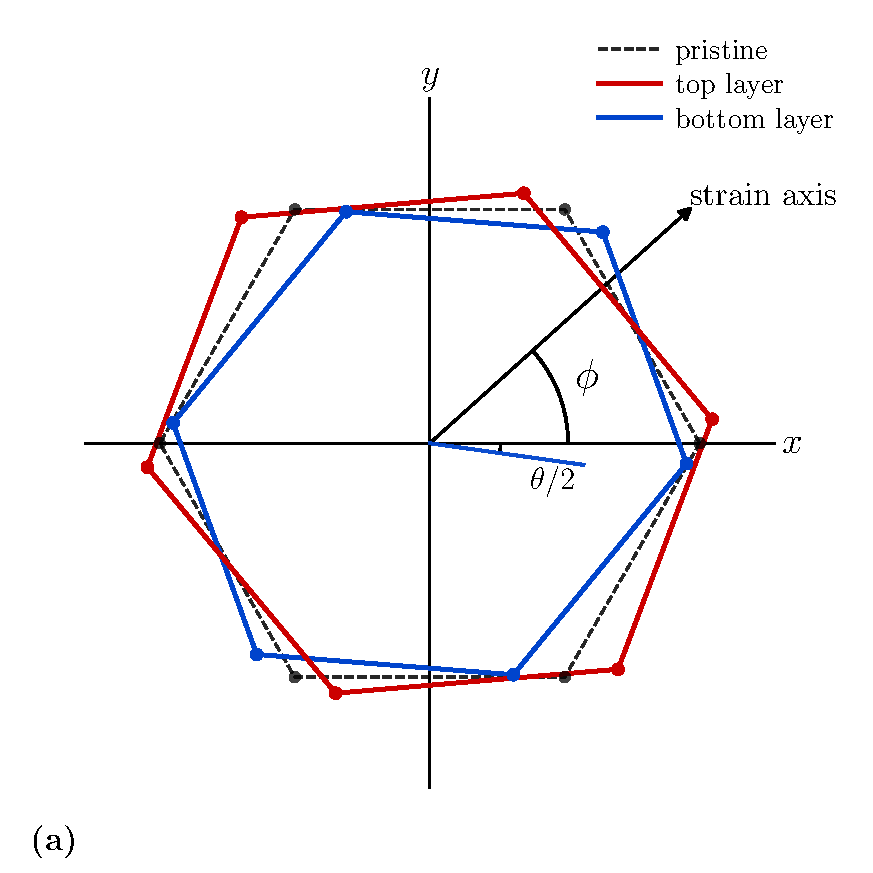
\includegraphics[width=0.45\textwidth]{fig/2/hetero_hexagon.pdf}
		&
		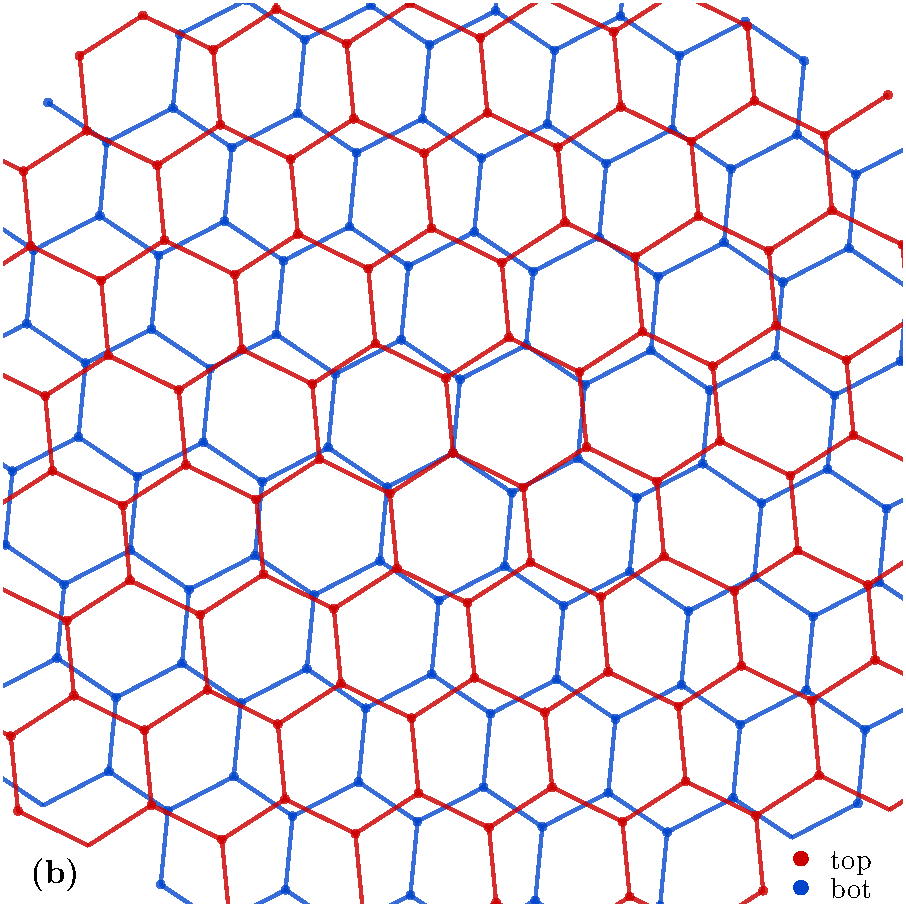
\includegraphics[width=0.45\textwidth]{fig/2/hetero_honeycomb.pdf}
	\end{tabular}
	\caption{
		Schematic of TBG under heterostrain.
	(a) A Brillouin zone before and after applying opposite layer rotations and heterostrain. The dashed black hexagon denotes the pristine BZ, while red and blue denote the top and bottom layers.
	(b) Top-view honeycomb lattice of TBG under heterostrain. 
	}
	\label{fig2}
\end{figure}

The geometry of each layer of TBG under a uniform deformation in real space can be described by
\begin{align}
	\bm{r}^\pr = \p{\mr{I}_{2 \times 2} + \mathcal{E}} \bm{r},
\end{align}
where \(\mathcal{E}\) is two-dimensional deformation matrix containing the strain and rotation part. In the small-angle limit, it can be written as \(\mathcal{E} = \begin{pmatrix}
		\mathcal{S}_{xx} & \mathcal{S}_{xy} - \te\\
		\mathcal{S}_{yx} + \te & \mathcal{S}_{yy}
 	\end{pmatrix} = \mathcal{S}\p{\epsilon, \phi} + \mathcal{T} \p{\te}.\)
Here \(\mathcal{S}\) denotes the symmetric strain tensor, while \(\mathcal{T}\) denotes the antisymmetric rotation tensor. The two-dimensional strain tensor is
\begin{align}
	\mathcal{S} \p{\epsilon, \phi} = R \p{\phi} \begin{pmatrix}
		\epsilon_1 & \\
		& \epsilon_2
	\end{pmatrix} R^{T} \p{\phi} = \begin{pmatrix}
		\epsilon_1 \cos^{2} \phi + \epsilon_2 \sin^2 \phi  & \p{\epsilon_1 - \epsilon_2} \cos \phi \sin \phi\\
		\p{\epsilon_1 - \epsilon_2} \cos \phi \sin \phi & \epsilon_1 \sin^2 \phi + \epsilon_2 \cos^2 \phi
	\end{pmatrix},
\end{align}
where \(R \p{\phi}\) is also the rotation matrix (we use different label to describe the rotation of twist layer and the strain direction), \(\epsilon_1\) and \(\epsilon_2\) are the strain magnitudes and \(\phi\) is the strain direction. We take \(\epsilon_1=\epsilon\) and \(\epsilon_2=-\nu\epsilon\), where \(\nu=0.16\) is the Poisson ratio of graphene.

Correspondingly, the momentum is rescaled as
\begin{align}
	\bm{k}^\pr \cong \p{\mr{I}_{2 \times 2} - \mathcal{E}^{T}} \bm{k},
\end{align}
so that \(\bm{k}^\pr \cdot \bm{r}^\pr = \bm{k} \cdot \bm{r}\). The rescaled primitive and reciprocal lattice vectors are 
\begin{align}
	\bm{a}^{\pr}_{1/2} = \p{\mr{I}_{2 \times 2} + \mathcal{E}} \bm{a}_{1/2}, \quad \bm{b}^{\pr}_{1/2} \cong \p{\mr{I}_{2 \times 2} - \mathcal{E}^{T}} \bm{b}_{1/2}.
\end{align}

For heterostrain, the two layers are taken to have opposite strain magnitudes but the same strain direction. We take the parameters in strain tensors of the top and bottom layers to be \(\mathcal{S}_{t}\p{\frac{\epsilon}{2}, \phi}\) and \(\mathcal{S}_{b}\p{-\frac{\epsilon}{2}, \phi}\). The rotation tensors are \(\mathcal{T}_{t} \p{\te/2}\) and \(\mathcal{T}_{b} \p{-\te/2}\). So the deformation matrices for the top and bottom layers are \(\mathcal{E}_{t} = \mathcal{S}_{t} + \mathcal{T}_{t}\) and \(\mathcal{E}_{b} = \mathcal{S}_{b} + \mathcal{T}_{b}\).

Like the geometric relationship, the geometric relationship of reciprocal lattice vectors in the moiré system under heterostrain has the similar form which is 
\begin{align}
	\bm{b}^{\prime}_{m; 1/2} = \p{\mathcal{E}_{t} - \mathcal{E}_{b}}^{T} \bm{b}_{1/2} = \p{\mathcal{S} + \mathcal{T}}^{T} \bm{b}_{1/2},
	\quad
	\bm{q}^{\prime}_{1} = \p{\mathcal{E}_{t} - \mathcal{E}_{b}}^{T} \bm{K} = \p{\mathcal{S} + \mathcal{T}}^{T} \bm{K}.
\end{align}


\subsection{Hamiltonian under Heterostrain}
The Hamiltonian of TBG under heterostrain is \(H^{\pr}_{t/b} = v_F \bm{p}^\pr \cdot \bm{\sigma} \pm \p{\alpha \vph I_{\mr{2 \times 2}} + v_F \gamma \bm{A} \cdot \bm{\sigma}}\) and \(\bm{p}_{t}^\pr = \bm{k} - \p{n_1 \bm{b}^{\pr}_{m;1} + n_2 \bm{b}^{\pr}_{m;2}}\) and \(\bm{p}_{b}^\pr = \bm{k} - \p{\bm{q}^{\prime}_{1} + n_1 \bm{b}^{\pr}_{m;1} + n_2 \bm{b}^{\pr}_{m;2}}\) are the relative momentum under heterostrain. The effect of heterostrain enters the continuum Hamiltonian through three contributions. First, it deforms the geometry of the moir\'e reciprocal lattice and hence modifies the momenta in the intralayer Dirac Hamiltonian \(\bm{p} \rightarrow \bm{p}^\prime\). Second, it generates a pseudoscalar field \(\vph\), which enters as a layer-dependent scalar potential. Third, it induces a pseudovector field \(\bm A\), which couples to the Dirac fermions through the sublattice Pauli matrices.

With the geometric relationship above, we rewrite the intralayer Hamiltonian as
\begin{align}
	\begin{split}
		H^{\pr}_{b} & = v_{F} \hbar \bb{\bm{k} -  \p{\mathcal{S} + \mathcal{T}}^{T} \p{\bm{K} + n_1 \bm{b}_{1} + n_2 \bm{b}_{2}} } \cdot \bm{\sigma} - \alpha \vph \mr{I}_{2 \times 2} - v_F \gamma \bm{A} \cdot \bm{\sigma}, \\
		H^{\pr}_{t} & = v_{F} \hbar \bb{\bm{k} -  \p{\mathcal{S} + \mathcal{T}}^{T} \p{n_1 \bm{b}_{1} + n_2 \bm{b}_{2}} } \cdot \bm{\sigma} + \alpha \vph \mr{I}_{2\times2} + v_F \gamma \bm{A} \cdot \bm{\sigma},
	\end{split}
\end{align}

The pseudoscalar field \(\vph\) and pseudovector field \(\bm{A}\) are defined as
\begin{align}
	\begin{split}
		\vph &= \mr{Tr}\p{\mathcal{S}} = \epsilon_1 + \epsilon_2 \\
	    \bm{A} &= \begin{pmatrix}
		    \mathcal{S}_{xx} - \mathcal{S}_{yy},&   \mathcal{S}_{xy} + \mathcal{S}_{yx}
	        \end{pmatrix}  = \begin{pmatrix}
		    \p{\epsilon_1 - \epsilon_2} \cos{2 \phi},&  \p{\epsilon_1 - \epsilon_2} \sin{2 \phi}
	        \end{pmatrix}.
	\end{split}
\end{align}

The interlayer tunneling part remains unchanged with BM model because the coefficient \(w_{3} \approx 10 \mr{meV}\) in the breaking p-h symmetry term \(i \sigma_3 w_3\) in Kang's paper is much smaller than \(w_0, \, w_1 \approx 100 \mr{meV}\) in the original BM model. 

The parameters in the BM model with heterostrain are listed in the following table.
\begin{table*}[h!]
	\centering
	\begin{tabular}{c c c c c c c}
		\toprule
		Parameter & \(v_{F} \hbar/a\) & \(w_0\) & \(w_1\) & \(\alpha\) & \(v_{F} \gamma\) & \(\nu\) \\
		\midrule
		value & \(2.4167  \mr{eV}\) & \(54.4  \mr{meV}\) &  \(124.9 \mr{meV}\) &  \(-1.0542 \mr{eV}\) &  \( -3.3644 \mr{eV}\) & \(0.16\) \\
		\bottomrule
	\end{tabular}
\end{table*}

After introducing heterostrain, the symmetry of the BM model is reduced. The threefold rotational symmetry \(C_{3z}\) and the layer-exchange symmetry \(C_{2x}\) are generally broken. As a result, the Dirac points are no longer pinned to the high-symmetry corners of the moir\'e Brillouin zone. However, the combined symmetry \(C_{2z}\mathcal{T}\) is still preserved, which protects the Dirac points from opening a gap. Moreover, the particle-hole symmetry remains valid since the system is still symmetric around the \(\bm{\Gamma}\) point.


\section{Evolution of Dirac points under heterostrian}
\subsection{Perturbative calculation of the shifted Dirac-point energy}
The introduction of heterostrain inherently breaks this \(C_{3z}\) symmetry and break the \(C_{2z}\) symmetry in mostly situation(and we will discuss in which situation the symmetry is respected). Since the symmetry is broken, the Dirac points are no longer pinned at the moir\'e Brillouin zone corners and can shift in momentum space. Moreover, the energetic degeneracy of the Dirac points is lifted, resulting in a shift in their energy. Calculating the strain-induced energy shift of the Dirac points is essential because it uncovers the microscopic origin of layer symmetry breaking, providing a direct theoretical link to the splitting of Van Hove singularities observed in STM experiments. We can treat the effects of heterostrain as a perturbation to the original BM Hamiltonian since the strain magnitude is very small (\(\epsilon \sim 0.1\%\)) and the shifted energy is corresponding to the first-order perturbation of the Hamiltonian. 

To obtain analytic expressions for the wavefunctions of Dirac points in original BM model, we truncate the Bloch-state basis to the 10 \(\bm{K}\) points in the first two shells, which yields a \(20\)-component basis. At the Dirac point in BM model, there are two wavefunctions degenerated at \(E = 0\). We denoted by \(\ket{\Phi} = \p{\ket{\phi_1}, \ket{\phi_2}}\). In this truncated basis, they can be written as
\begin{align}
	\ket{\phi_n} = \begin{pmatrix}
		\phi_{n,1}^{A} & \phi_{n,1}^{B} & \phi_{n,2}^{A} & \phi_{n,2}^{B} & \cdots & \phi_{n,10}^{A} & \phi_{n,10}^{B}
	\end{pmatrix}^T, \qquad n=1,2,
\end{align}
where \(n\) is the index of two wavefunctions and the index \(j=1,\dots,10\) labels the ten truncated basis.

\begin{figure}[h!]
	\captionsetup{list=false}
	\centering
	\begin{tabular}{c}
		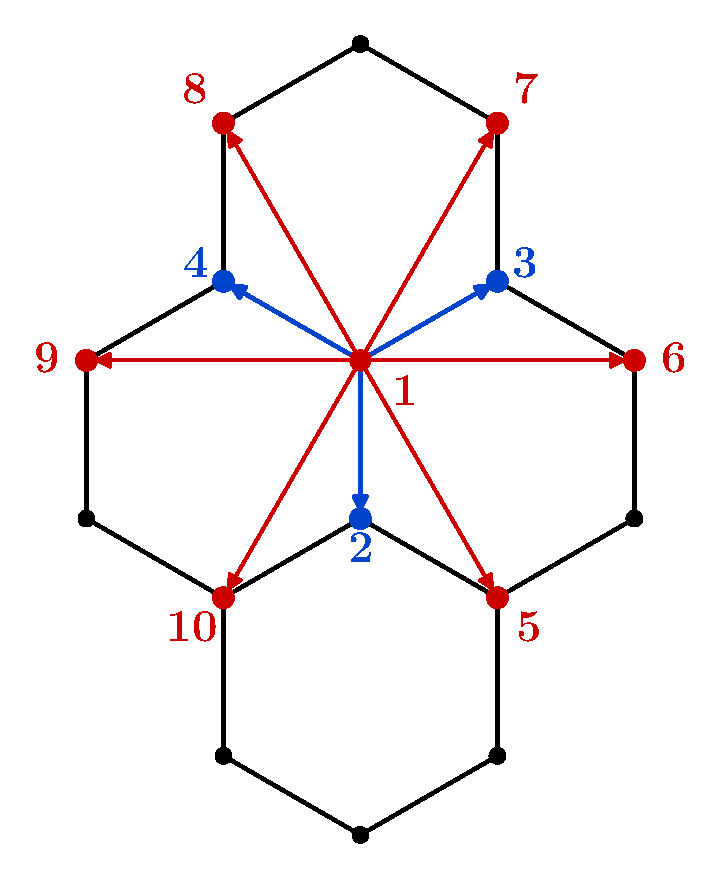
\includegraphics[width=0.3\textwidth]{fig/3/20by20.pdf}
	\end{tabular}
	\caption{Truncated momentum-space basis used for the analytical Dirac-point wavefunctions.
	}
	\label{fig3}
\end{figure}

By imposing the \(C_{3z}\) symmetry and solving the Schr\"odinger equation within this \(20\)-component basis, all components of the two Dirac-point eigenstates can be expressed in terms of one independent amplitude for each state. Choosing \(\phi_{1,2}^{A}=w_0\) for \(\ket{\phi_1}\) and \(\phi_{2,2}^{A}=w_1\) for \(\ket{\phi_2}\), we obtain two analytic eigenstates. For brevity, their explicit component expressions are given in Appendix~A.

The perturbation Hamiltonian is \(\delta H = H^{\pr} - H_{0}\). For the bottom layer, it is
\begin{align}
	\begin{split}
		\delta H_{b} = v_F \hbar \bb{ \bm{k} - \mathcal{S} \p{\bm{K} + n_1 \bm{b}_{1} + n_2 \bm{b}_{2}}} \cdot \bm{\sigma} - \alpha \vph \mr{I}_{2 \times 2} - v_F \gamma \bm{A} \cdot \bm{\sigma}.
	\end{split}
\end{align}
Where \(\mathcal{S}^{T} = \mathcal{S}\). For the top layer, it is
\begin{align}
	\begin{split}
		\delta H_{t}  = v_F \hbar \bb{\bm{k} - \mathcal{S} \p{n_1 \bm{b}_{1} + n_2 \bm{b}_{2}}}  \cdot \bm{\sigma} + \alpha\vph \mr{I}_{2\times2} + v_F\gamma\bm{A}\cdot\bm{\sigma}.		
	\end{split}
\end{align}
Projecting the perturbation onto the two-dimensional Dirac-point subspace gives the effective first-order perturbation matrix
\begin{align}
	H_{1}^{\mathrm{eff}}(\bm{k}) = \braket{\Phi|\delta H|\Phi}  = \begin{pmatrix}
		\braket{\phi_{1} | \delta H | \phi_{1}} & \braket{\phi_{1} | \delta H | \phi_{2}} \\
		\braket{\phi_{2} | \delta H | \phi_{1}} & \braket{\phi_{2} | \delta H | \phi_{2}}
	\end{pmatrix}.
\end{align}
Since \(C_{2z}\mathcal{T}\) is preserved, this effective Hamiltonian cannot contain a mass term proportional to \(\sigma_z\). Therefore, it can be written as \(H_{1}^{\mathrm{eff}}(\bm{k}) = h_0(\bm{k})\sigma_0 + h_x(\bm{k})\sigma_x + h_y(\bm{k})\sigma_y \). The two eigenvalues are \(E_{\pm}(\bm{k}) = h_0(\bm{k}) \pm \sqrt{ h_x^2(\bm{k}) + h_y^2(\bm{k})}\). The scalar part \(h_0(\bm{k})\) can be obtained from the trace of the projected perturbation matrix. At the shifted Dirac point, where \(h_x(\bm{k}_{\mr{DP}})=h_y(\bm{k}_{\mr{DP}})=0\), the Dirac-point energy is \(E_{\mr{DP}} = h_0(\bm{k}_{\mr{DP}})\). Evaluating the diagonal term using the analytical wavefunctions in Appendix~A gives the energy of shifted Dirac points
\begin{align}
		E_{\mr{DP}} &= \mathcal{N}^2 \Bigg\{ \alpha \vph \bb{\p{\frac{w_0^2}{v_{F} \hbar \bv{\bm{q}_1}} - v_{F} \hbar \bv{\bm{q}_1}}^2 - 3 \p{w_0^2 + w_1^2} + \frac{2}{ \p{v_{F} \hbar \bv{\bm{q}_1}}^2} \p{w_0^4 + w_1^4 + 4 w_0^2 w_1^2}}\\
		&+ \vph w_0 w_1 \frac{4 \pi}{a}  \bb{v_{F} \hbar + \frac{1}{v_{F} \hbar \bv{\bm{q}_{1}}^2} \p{-2 w_0^2 - w_1^2}} \Bigg\}.
\end{align} 
Here \(\mathcal{N}\) is the normalization coefficient of wavefunctions defined in Appendix~A. By particle-hole symmetry, the corresponding energy of Dirac point in the other layer is \(-E_{\mr{DP}}\).

The off-diagonal terms determine the linear dispersion around the shifted Dirac point. In the present approximation, the renormalized velocities are given by the coefficients of \(k_x\) and \(k_y\)
\begin{align}
	v^{*}_{x} = v^{*}_{y} =v_{F} \mathcal{N}^2 \p{ -2 w^{2}_0 - 3 w^{2}_1+ v_{F}^2 \hbar^2 \bv{\bm{q}_{1}}^2 + \frac{2 w_0^4 + 4 w_0^2 w_1^2 + w_1^4}{v_{F}^2 \hbar^2 \bv{\bm{q}_{1}}^2}}.
\end{align}
Therefore, although the velocity is renormalized from the bare value \(v_F\), the Dirac cone remains isotropic at this order.


\subsection{Numerical result}
The positions of the shifted Dirac points under heterostrain can be identified as the points where the gap between the two bands vanishes.
We first calculate the distribution of the energy gap between the two central flat bands under heterostrain at a fixed twist angle \(\theta = 1.40^{\circ}\). Here, we set the momentum is normalized by length unit \(G_m \equiv |\bm{b}_{m,1}| = \frac{8\pi\sin(\theta/2)}{\sqrt{3}a}\).

\begin{figure}[h!]
	\captionsetup{list=false}
	\centering
	\begin{tabular}{cc}
		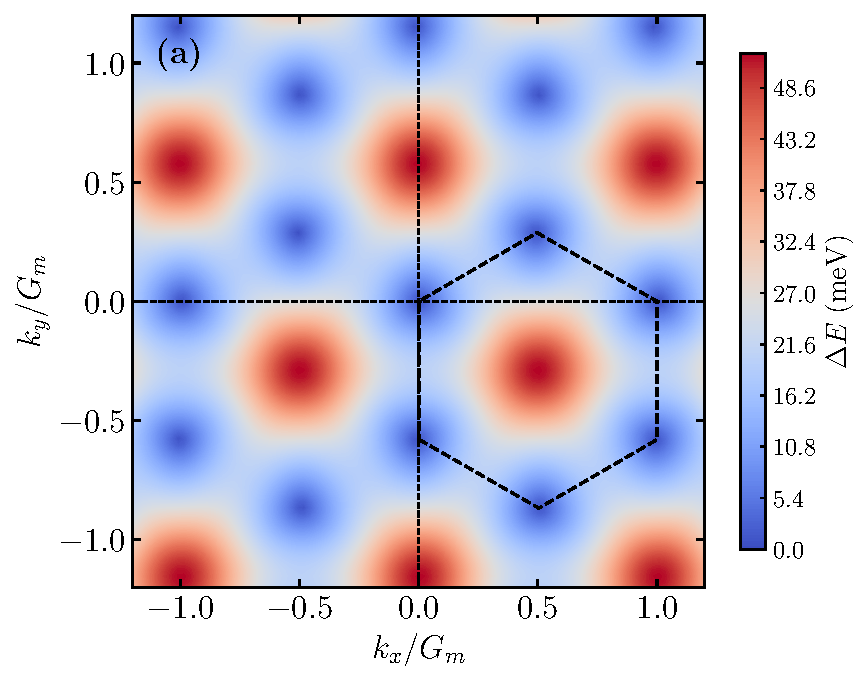
\includegraphics[width=0.45\textwidth]{fig/4/phi_10_ep_001_gap.pdf}
		&
		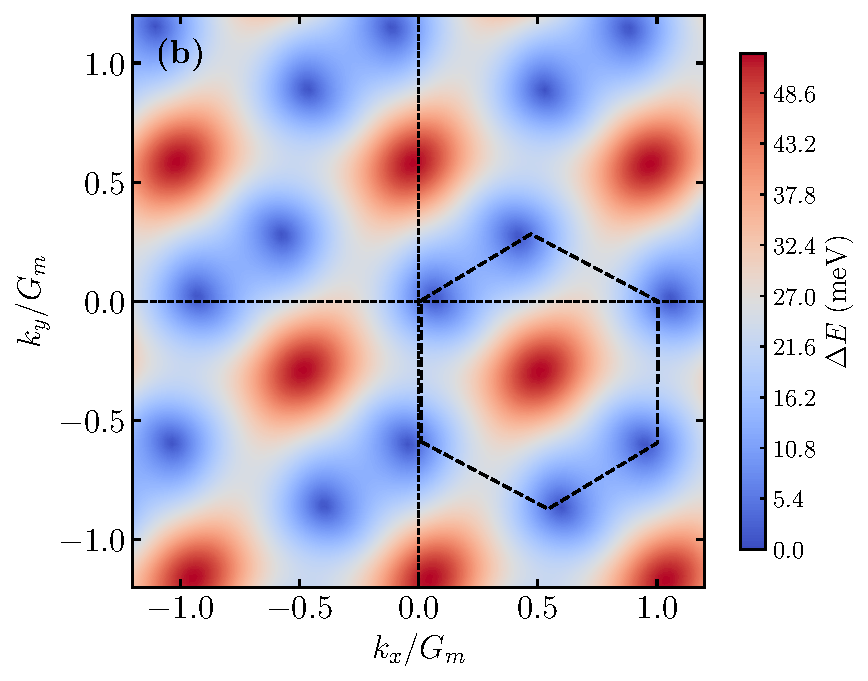
\includegraphics[width=0.45\textwidth]{fig/4/phi_10_ep_01_gap.pdf}
	\end{tabular}
	\caption{
		Gap distribution between the two central flat bands for \(\phi=10^\circ\).
	(a) \(\epsilon=0.01\%\).
	(b) \(\epsilon=0.1\%\).
	The dashed hexagon denotes the strained moir\'e Brillouin zone.
	}
	\label{fig4}
\end{figure}

We next examine the effective ratio \(E_{\mathrm{DP}}/\epsilon\). As shown in Fig.~\ref{fig5}(a), the ratio exhibits a clear angular dependence with period \(\pi/3\). For small \(\epsilon\), the angular modulation is weak, consistent with the leading linear response. As \(\epsilon\) increases, the modulation becomes much stronger, indicating sizable higher-order corrections controlled by the strain direction.

Figure~\ref{fig5}(b) shows \(E_{\mathrm{DP}}/\epsilon\) as a function of \(\epsilon\) for several fixed strain directions \(\phi\). The energy shift is linear  only to leading order in small \(\epsilon\) regime; for larger \(\epsilon\), it acquires a significant nonlinear correction, whose magnitude and sign also depend on the strain direction \(\phi\).

\begin{figure}[h!]
	\captionsetup{list=false}
	\centering
	\begin{tabular}{ccc}
		
\includegraphics[width=0.30\textwidth]{fig/5/comp_epsilon.pdf}
		&
		
\includegraphics[width=0.30\textwidth]{fig/5/comp_phi.pdf}
		&
		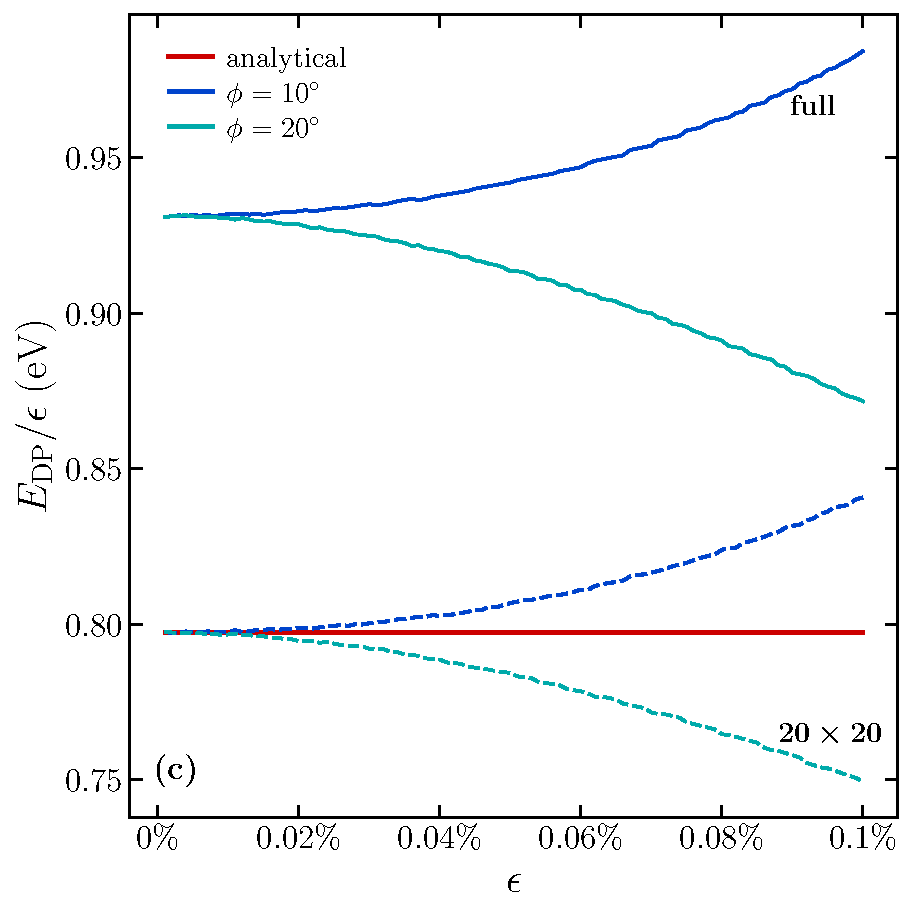
\includegraphics[width=0.30\textwidth]{fig/5/comp_an.pdf}
	\end{tabular}
	\caption{
		Ratio \(E_{\mathrm{DP}}/\epsilon\) as a function of heterostrain parameters.
	(a) Dependence on the strain direction \(\phi\) for fixed \(\epsilon\).
	(b) Dependence on the strain magnitude \(\epsilon\) for fixed \(\phi\).
	(c) Comparison between the analytical perturbative result, the full numerical calculation, and the \(20\times20\) truncated-basis calculation.
	In (c), solid and dashed curves denote the full and \(20\times20\) numerical results, respectively.
	}
	\label{fig5}
\end{figure}

\begin{itemize}
	\item Error analysis
\end{itemize}

In Fig.~\ref{fig5}(c), we compare the analytical perturbative result with both the large truncated \(324\times324\) Hamiltonian and the small truncated \(20\times20\) Hamiltonian. The full \(324\times324\) results differs from both the \(20\times20\) and analytical results by roughly \(10 \sim 15\%\). For small \(\epsilon\p{0 \sim 0.02\%}\), the difference between the \(20\times20\) calculation and the analytical result becomes negligible.

Indeed, projecting the large-scale numerical eigenstates onto the first 20 basis components gives a weight of about \(0.9\), while the remaining higher-shell components carry about \(0.1\). Although this residual weight is small, it can still affect the energy shift because the strain perturbation contains intralayer terms proportional to \(\mathcal S(\bm K+\bm G)\). These terms become larger for higher momentum shells, so the high-\(|\bm G|\) components can contribute appreciably to the first-order perturbative energy. Therefore, the error in \(E_{\mathrm{DP}}/\epsilon\) can reach \(10\%\sim15\%\) even when the wave-function weight outside the \(20\times20\) subspace is only about \(10\%\).

% \begin{figure*}[h!]

% 	\centering
% 	\begin{subfigure}[t]{0.30\linewidth}
% 		\centering
% 		
\includegraphics[width=\linewidth]{pic/further/comp_epsilon.pdf}
% 		\caption{\(E_{\mr{DP}}/\epsilon\) vs \(\phi\)}
% 		\label{fig:edp_phi}
% 	\end{subfigure}
% 	\hspace{0.04\linewidth}
% 	\begin{subfigure}[t]{0.30\linewidth}
% 		\centering
% 		
\includegraphics[width=\linewidth]{pic/further/comp_phi.pdf}
% 		\caption{\(E_{\mr{DP}}/\epsilon\) vs \(\epsilon\)}
% 		\label{fig:edp_epsilon}
% 	\end{subfigure}
% 	\caption{\(E_{\mr{DP}}/\epsilon\) with different \(\epsilon\) and \(\phi\).}
% 	\label{fig:edp_scaling}

% \end{figure*}

\subsection{Beyond Perturbation}

By symmetry, the uniaxial strain tensor satisfies
\begin{align}
	\mathcal S(\epsilon,\phi+\pi)=\mathcal S(\epsilon,\phi).
\end{align}
On the other hand, the pristine BM Hamiltonian has the threefold rotational symmetry \(C_{3z}\), which relates configurations whose strain directions differ by \(2\pi/3\). Consequently, the energy of shifted Dirac points must satisfy
\begin{align}
	E_{\mr{DP}}(\epsilon,\phi+\pi/3)
	=
	E_{\mr{DP}}(\epsilon,\phi).
\end{align}
Thus, the leading angular dependence can only appear through the sixth harmonic, such as \(\cos 6\phi\) and \(\sin 6\phi\). This can be understood from pseudovector field \(\bm{A}\), which depends on the strain angle as \(\bm{A} \sim (\cos 2\phi, -\sin 2\phi)\). Since the first-order perturbation Hamiltonian contributes linearly in \(\epsilon\), a nonzero angular dependence of the energy appears only at third order in \(\epsilon\).

We therefore expand the energy of the top-layer Dirac points as
\begin{align}
	E^{t}_{\mr{DP}}  = A \epsilon + B \epsilon^{2} + \epsilon^3 \p{C_1 + C_{2} \cos{6 \phi} + C_{3} \sin{6 \phi}} + O\p{\epsilon^{4}},
\end{align}
Here the first two terms are independent of \(\phi\), while the leading angular modulation appears at order \(\epsilon^3\). This form is consistent with the \(\pi/3\)-periodicity in the strain direction.

Particle-hole symmetry relates the two layer-related Dirac points and reverses the sign of the energy, 
\begin{align}
	E^{b}_{\mr{DP}}  = - A \epsilon - B \epsilon^2 - \epsilon^3 \p{C_{1} + C_{2} \cos{6 \phi} + C_{3} \sin{6 \phi}} + O\p{\epsilon^{4}}.
\end{align}
In addition, the layer-exchange operation \(C_{2x}\) also relates the Dirac points in the top and bottom layers. Under the \(C_{2x}\) operation, the strain configuration is transformed as \((\epsilon,\phi)\rightarrow(-\epsilon,-\phi)\). Thus, \(E_{\mr{DP}}^{b}(\epsilon,\phi) = E_{\mr{DP}}^{t}(-\epsilon,-\phi)\). Using the expansion above, the right-hand side becomes
\begin{align}
	E_{\mr{DP}}^{b}(\epsilon,\phi) = E_{\mr{DP}}^{t}(-\epsilon,-\phi) = -A\epsilon + B\epsilon^2 - \epsilon^3 \p{ C_1 + C_2\cos 6\phi - C_3\sin 6\phi} + O(\epsilon^4).
\end{align}
Comparing this expression with the particle-hole relation for \(E_{\mr{DP}}^{b}(\epsilon,\phi)\), we obtain \(B=C_3=0\). Therefore, the symmetry-allowed form of the energy is
\begin{align}
		\frac{E_{\mr{DP}}^{t}(\epsilon,\phi)}{\epsilon} = A + \epsilon^2 \p{ C_1 + C_2\cos 6\phi } + O(\epsilon^3).
\end{align}
By fitting the numerical data of \(E_{\mr{DP}}/\epsilon\), we obtain the coefficients 
\begin{align}
	A = 0.9306~\mathrm{eV}, \qquad
	C_1 = -1.48\times10^{4}~\mathrm{eV}, \qquad
	C_2 = 1.11\times10^{5}~\mathrm{eV}.
\end{align}
The coefficients satisfy \(|C_2| \gg |C_1|\), showing that the dominant higher-order correction is strongly anisotropic and controlled by the \(\cos6\phi\) harmonic.


\subsection{Dirac point merging}
A special situation arises when the Hamiltonian preserves the \(C_{2x}\) symmetry. In the \(\bm{\Gamma}_m\)-centered convention, A Dirac points in top layer with position \(k_x, k_y\) will be mapped to a Dirac point in the bottom layer with position \(k_x, 2 \bm{\Gamma}_{m;y} - k_y\) under the \(C_{2x}\) operation. 

So under \(C_{2x}\) symmetry, the motion of two Dirac points is constrained in a single symmetry line(\(k_y\) axis). By tuning the parameters, i.e. heterostrain magnitude \(\epsilon\) and direction \(\phi\), we can change the \(k_y\) value of one Dirac point(\(\bm{K}_{t}\)) and the corresponding two Dirac points can be brought together and merged on this line.

The \(C_{2x}\) symmetry condition can be written as
\begin{align}
	H(C_{2x}\bm{k}) = U_{C_{2x}} H(\bm{k}) U_{C_{2x}}^\dagger,
\end{align}
with \(U_{C_{2x}}=\tau_x\otimes\sigma_x\). Applying this condition to the Hamiltonian under heterostrain shows that the pseudoscalar term must vanish and that the pseudovector field must be parallel to the \(k_y\) axis. In our parametrization, this requires \(\varphi = 0,\,A_x = 0,\)
or equivalently
\begin{align}
	\epsilon_1=-\epsilon_2 \Leftrightarrow \nu = 1,
	\qquad
	\phi=\p{\frac{n}{2} + \frac{1}{4}} \pi.
\end{align}

The detailed derivation is given in Appendix~B. In the present convention, the direction of motion is determined by the sign of \(A_y\) together with the fact that the coefficient \(\gamma\) is negative. As a result, although both \(\phi=45^\circ\) and \(\phi=135^\circ\) satisfy the condition \(A_x=0\), they correspond to opposite trajectories in \(k_y\) direction. For \(\phi=45^\circ\), the top-layer Dirac point moves toward \(+k_y\) while the bottom-layer Dirac point moves toward \(-k_y\), so the two Dirac points move away from each other. By contrast, for \(\phi=135^\circ\), the two Dirac points move toward each other along the \(k_y\) axis and can therefore merge at the midpoint of \(\bm q_1\). It's clear that the position of the \(\bm{q}_1\) will change with the \(\epsilon\) increasing while only the origin is fixed under hereostrain. Numerically, for \(\phi=135^\circ\), as \(\epsilon\) increases from small values, the two Dirac points first move longitudinally toward each other and merge near the midpoint of \(\bm q_1\) at zero energy for \(\epsilon \approx 0.1635 \% \sim 0.1642 \%\).  

\begin{figure}[h!]
	\captionsetup{list=false}
	\centering
	\begin{tabular}{c}
		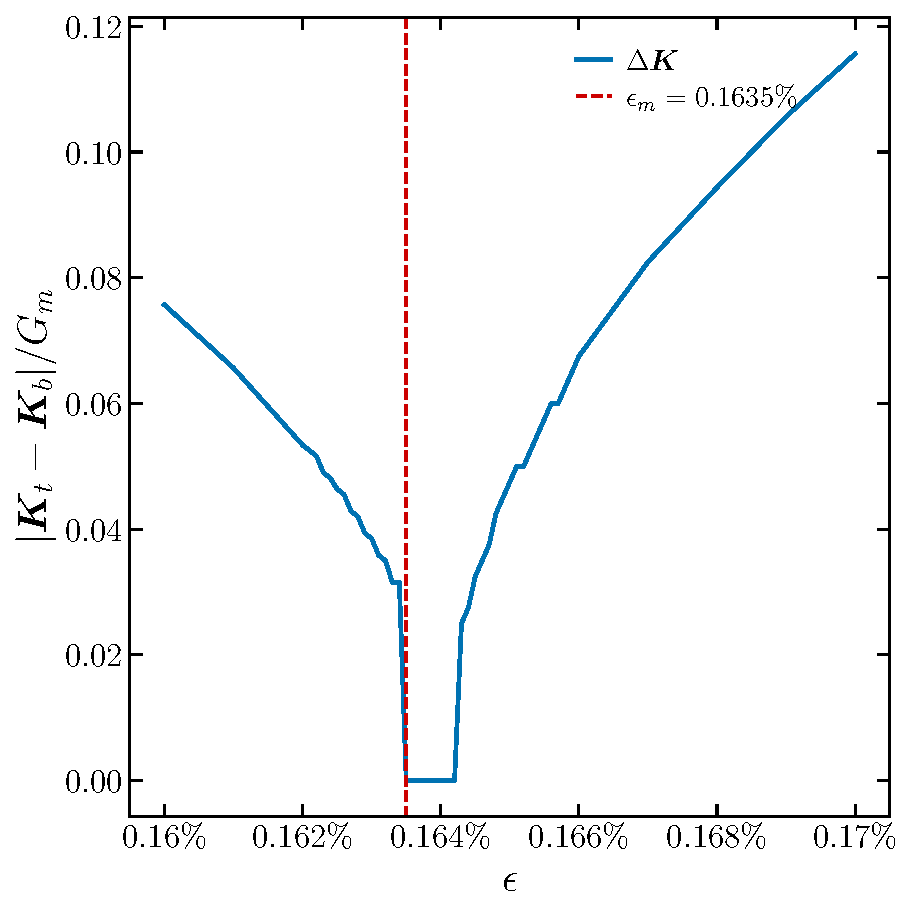
\includegraphics[width=0.40\textwidth]{fig/6/merge.pdf}
	\end{tabular}
	\caption{
		Distance between two Dirac points versus heterostrain magnitude $\epsilon$. The dashed line marks $\epsilon_m=0.1635\%$.
	}
	\label{fig6}
\end{figure}


\section{Van Hove singularity splitting}
\subsection{DOS configuration and evolution of VHS}
A van Hove singularity (VHS) arises from a saddle point of the band dispersion. For the \(n\)-th band, it is located at momenta satisfying \(\nabla_{\bm{k}} E_n(\bm{k}) = 0\), with a negative determinant of the Hessian matrix of \(E_n(\bm{k})\). Such points produce divergent peaks in the density of states (DOS), thereby enhancing electronic interactions and promoting correlated phenomena.

In monolayer graphene, the relevant saddle points are located at the \(\bm{M}\) points, i.e., the midpoints of the edges of the hexagonal Brillouin zone, with their positions fixed by the \(C_{2x}\) and \(C_{2y}\) symmetries. However, in twisted bilayer graphene, \(C_{2y}\) is broken whereas \(C_{2x}\) is retained. As a result, the VHS of the moiré flat bands are not pinned exactly to the edge midpoints of the moiré Brillouin zone. Although the VHS are no longer pinned at the \(\bm{M}\) points, they remain close to the high-symmetry points since the twist angle is small.

\begin{figure}[h!]
	\captionsetup{list=false}
	\centering
	\begin{tabular}{ccc}
		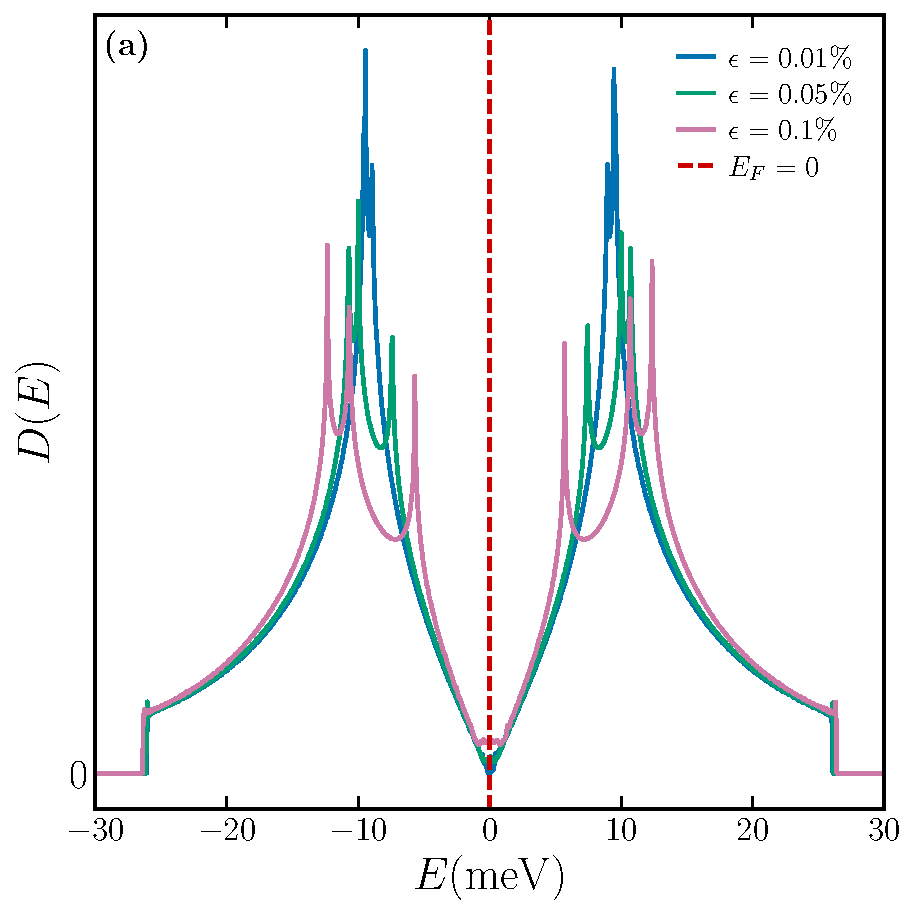
\includegraphics[width=0.30\textwidth]{fig/7/dos.pdf}
		&
		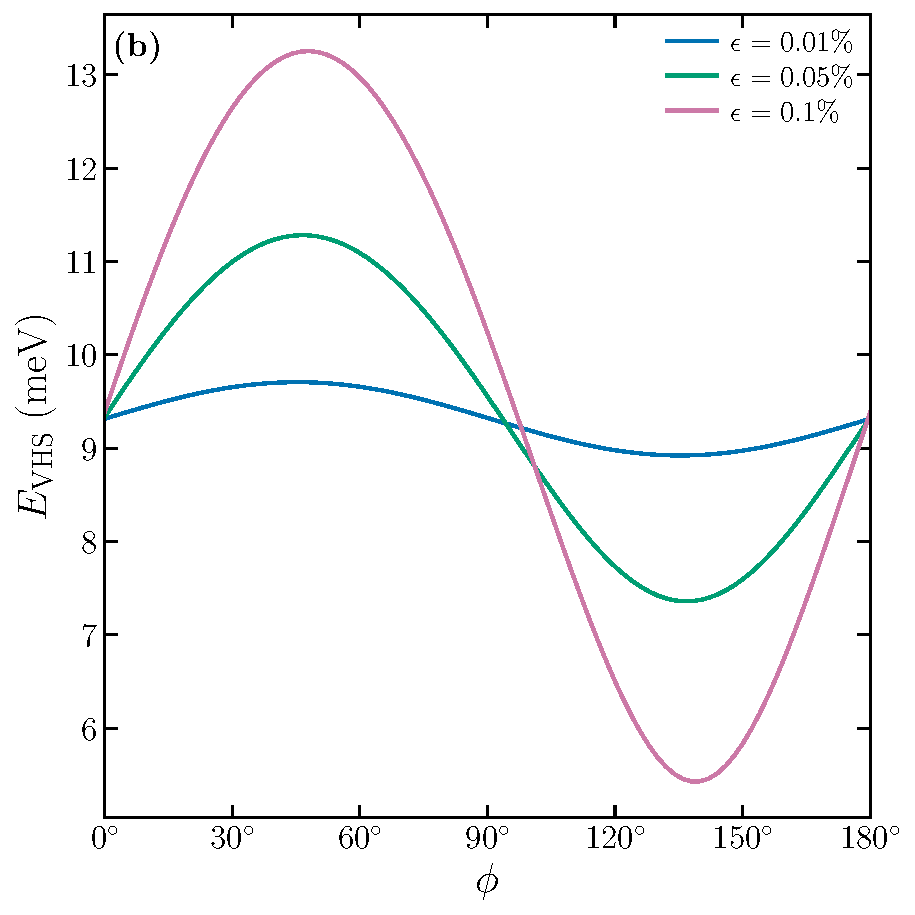
\includegraphics[width=0.30\textwidth]{fig/7/vhs1_energy_vs_phi.pdf}
		&
		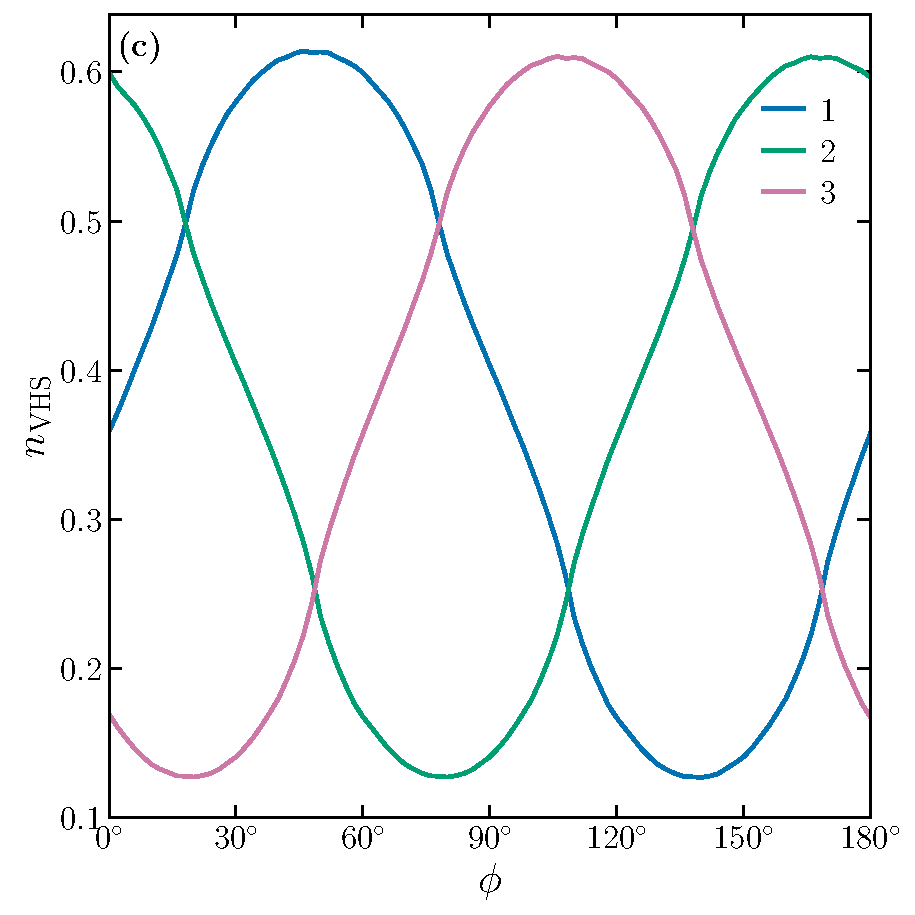
\includegraphics[width=0.30\textwidth]{fig/7/phi_vs_n_new.pdf}
	\end{tabular}
	\caption{
		Evolution of van Hove singularities under heterostrain.
        (a) Density of states $D(E)$ near charge neutrality for several strain magnitudes $\epsilon$ at fixed strain direction $\phi$. The vertical dashed line marks $E_F=0$. Heterostrain splits and shifts the flat-band van Hove peaks.\
        (b) Angular dependence of the VHS energy $E_{\rm VHS}$ as the strain direction $\phi$ is varied. The amplitude of the oscillation increases with the strain magnitude $\epsilon$.\
        (c) Carrier density $n$ evaluated at the VHS energies. The three branches labeled $1,2,3$ correspond to the three VHS trajectories in panel (b), showing the strain-direction-dependent redistribution of VHS-associated carrier densities.
	}
	\label{fig7}
\end{figure}


The heterostrain breaks \(C_{3z}\) and consequently splits the originally degenerate VHS, which is directly manifested as triple peaks in the DOS. Unlike the energy of shifted Dirac points, the energy of shifted VHS are difficult to obtain analytically. We therefore extract the VHS energies numerically. For each set of heterostrain parameters \(\p{\epsilon, \phi}\), we search the higher flat band for the saddle points satisfying \(\nabla_{\bm{k}}E_n(\bm{k})=0\). We denote these extracted VHS energies as \(E_{\mr{VHS}}\). The energy of three VHS of the lower flat band can be obtained by the particle-hole symmetry.

Although the VHS splitting is naturally described in energy, it is often more useful experimentally to express it in terms of carrier density \(n\). Since the Fermi level is typically tuned by doping, the relevant control parameter is the filling rather than the absolute energy. We therefore define \(n_{\mathrm{VHS}}\) as the carrier density at which the Fermi level reaches a VHS. This provides a more direct connection to transport and quantum-oscillation measurements, and shows at which fillings the Fermi-surface topology changes as the strain direction is varied.

We present the evolution result of the VHS under heterostrain. As shown in the density of states(DOS) in Fig.~\ref{fig7}(a), the heterostrain breaks the \(C_{3z}\) symmetry of the moir\'e superlattice and splits the originally degenerate VHS into three distinct peaks. Fig.~\ref{fig7}(b) shows the angular dependence of the VHS energies. The energy oscillation amplitude increases with \(\epsilon\) and exhibits a strict \(\pi\) periodicity. This originates from the fundamental geometric nature of the heterostrain tensor which depends on \(2 \phi\). Fig.~\ref{fig7}(c) shows the \(\phi\)-dependence of the carrier density \(n_{\mathrm{VHS}}\) corresponding to the VHS energy. The three split VHS are labeled as branches \(1,2,3\). For a given strain magnitude \(\epsilon\), the trajectories of the three VHS branches exhibit a precise \(\pi/3\) phase shift relative to one another. This phase difference can be derived directly from the \(C_{3z}\) symmetry of the unstrained system together with the \(2\phi\) dependence of the heterostrain Hamiltonian \(H'(\epsilon,\phi)\).

Let \(\ket{\phi_1}\) be the eigenstates of one VHS point in the pristine system. The other two energy-degenerate VHS points are related by \(C_{3z}\) symmetry and can be denoted as \(\ket{\phi_2} = C_{3z} \ket{\phi_1}\) and \(\ket{\phi_3} = C_{3z}^2 \ket{\phi_1}\). When the heterostrain is applied, the first-order energy shift of the first VHS point are given by \(\Delta E_1 \p{\phi} = \braket{\phi_1 | H_{1} | \phi_1}\). For the second VHS point, the energy shift is 
\begin{align}
	\Delta E_2 \p{\phi} = \braket{\phi_2 | H_{1} | \phi_2} = \braket{\phi_1 | C_{3z}^\dagger H_{1} C_{3z} | \phi_1} = \braket{\phi_1 | H_{1}(\epsilon, \phi + 2\pi/3) | \phi_1} = \Delta E_1(\phi - 2\pi/3).
\end{align}
Crucially, as discussed above, the heterostrain Hamiltonian is fundamentally a function of \(2 \phi\). Assuming the leading term of energy shift follows the form \(\Delta E_{1} \p{\phi} \propto \cos\p{2 \phi + \delta}\) where \(\delta\) is an initial phase offset dependent on the specific basis choice. Substituting this form into the symmetry relation yields
\begin{align}
	\Delta E_2 \p{\phi} \propto \cos \bb{2 \p{\phi - \frac{2 \pi}{3} + \delta}} =  \cos\bb{2 \p{\phi + \frac{\pi}{3}} +  \delta}.
\end{align}
This demonstrates the \(2 \pi/3\) spatial rotation of the wavefunctions combined with the \(2 \phi\) dependence of the heterostrain Hamiltonian leads to a \(\pi/3\) phase shift in the angular dependence of the VHS energy shifts.

\subsection{Quantum oscillation: Fermi surface and pocket area}

Heterostrain splits the three VHS by breaking \(C_{3z}\), and this splitting has direct consequences for the Fermi-surface topology and the associated quantum-oscillation frequencies. In the absence of heterostrain, the three VHS are degenerate. Once heterostrain is introduced, the three saddle points shift to different energies. As a result, the Fermi surface is reconstructed through a sequence of distinct Lifshitz transitions as \(E_F\) is varied, rather than through a single simultaneous transition.

Figure~\ref{fig8} illustrates this effect for fixed \(\epsilon=0.1\%\). At \(\phi=40^\circ\), the VHS energies are ordered as \(E_3<E_2<E_1\), whereas at \(\phi=60^\circ\) the ordering becomes \(E_2<E_3<E_1\). Thus, changing the strain direction \(\phi\) changes the order in which the VHS energies are crossed, and hence changes the sequence of Fermi-surface reconstructions.

For the representative case shown in Fig.~\ref{fig8}, as \(E_F\) increases, an electron pocket first expands around the \(\bm{K}\) point and remains electron pocket crossing the first two VHS energies. Between the second and third VHS energies, the contours reconnect into open Fermi surface. Only after crossing the third VHS does the Fermi surface evolve into a hole pocket. In other words, the reconstruction proceeds as
\[
\text{electron pocket} \;\rightarrow\; \text{electron pocket} \;\rightarrow\; \text{open Fermi surface} \;\rightarrow\; \text{hole pocket}.
\]
In the semiclassical magnetotransport picture, the appearance of open Fermi-surface segments implies open orbits, which naturally lead to the non-saturating quadratic \(\p{B^2}\) magnetoresistance observed experimentally.

\begin{figure}[h!]
	\captionsetup{list=false}
	\centering
	\begin{tabular}{cc}
		
\includegraphics[width=0.40\textwidth]{fig/8/ep_01_phi_40.pdf}
		&
		
\includegraphics[width=0.40\textwidth]{fig/8/ep_01_phi_60.pdf}
	\end{tabular}
	\caption{
		Fermi-surface contours at the split VHS energies for fixed \(\epsilon=0.1\%\) with different \(\phi\). The VHS ordering changes from \(E_3<E_2<E_1\) at \(\phi=40^\circ\) to \(E_2<E_3<E_1\) at \(\phi=60^\circ\). Thus, the strain direction controls the sequence of saddle-point reconnections, or equivalently the order of the VHS-induced Lifshitz transitions.
	}
	\label{fig8}
\end{figure}

In the energy window between the two shifted Dirac points, the Fermi surface contains both an electron pocket and a hole pocket. Denoting the  energies of shifted Dirac points by \(+E_0\) and \(-E_0\), a Fermi level satisfying \(-E_0<E_F<E_0\) cuts one Dirac cone above its node and the other below its node. As \(E_F\) increases within this window, the electron pocket expands while the hole pocket shrinks. Equivalently, when the carrier density is tuned from negative to positive values, the two pocket areas evolve in opposite directions. The two individual areas \(S_1\) and \(S_2\) exchange their relative weights across charge neutrality, while their sum \(S_{\mr{tot}}\) remains finite and reaches a minimum near \(n=0\). This behavior reflects the coexistence of electron-pocket and hole-pocket between the two shifted Dirac points.

\begin{figure}[h!]
	\captionsetup{list=false}
	\centering
	\begin{tabular}{cc}
		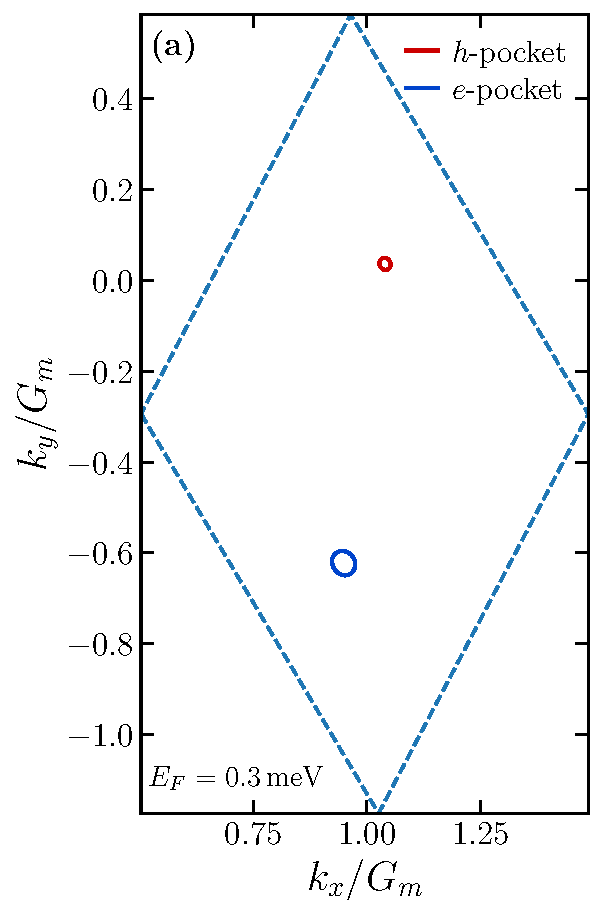
\includegraphics[width=0.30\textwidth]{fig/9/rpc_pocket.pdf}
		&
		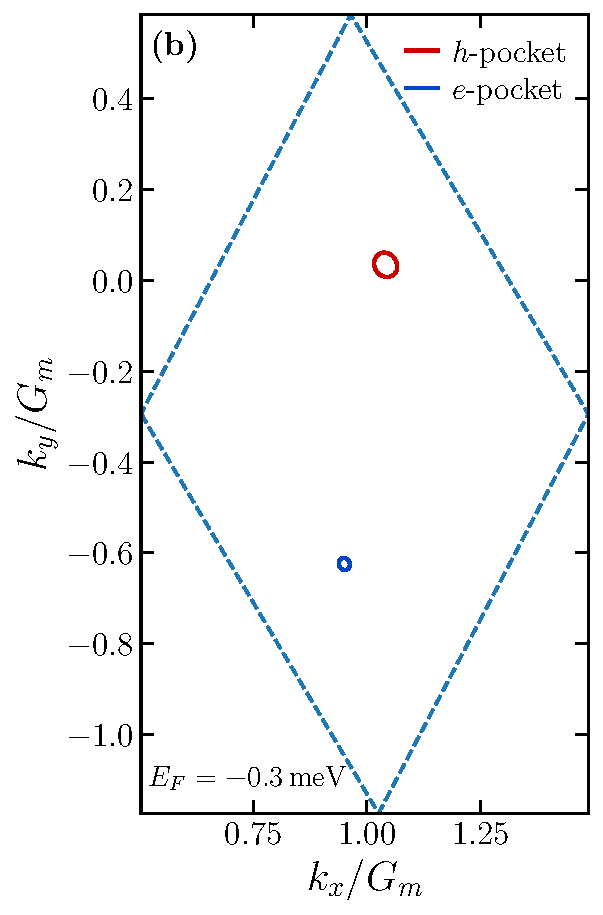
\includegraphics[width=0.30\textwidth]{fig/9/n_rpc_pocket.pdf}
	\end{tabular}
	\caption{
		Fermi-surface contours in the two-pocket regime between the shifted Dirac points. 
	}
	\label{fig9}
\end{figure}

The previous discussion focused on the qualitative evolution of the Fermi surface over a broad energy range. We now turn to the small-energy regime near the shifted Dirac points, where the pocket areas can be analyzed quantitatively. Because the shifted Dirac cones remain isotropic to first order in perturbation theory, the corresponding pocket areas can be obtained within an isotropic two-Dirac-cone approximation. These areas are directly relevant to quantum oscillations through the Onsager relation.

Within an isotropic two-Dirac-cone approximation, the total area of the coexisting pockets can be written as

\begin{align}
	S_{\mathrm{tot}} = \frac{2 \pi E_0^2}{\hbar^2 v_F^2}  + \frac{n^2 \hbar^2 v_F^2}{8 \pi E_0^2}.
\end{align}

The relation between the pocket areas and the carrier density is shown in Fig.~\ref{fig10}. The total area \(S_{\mr{tot}}\) is nonzero at charge neutrality because the two shifted Dirac points lie at different energies, and reaches a minimum there. As the carrier density \(n\) increases, the total area grows quadratically in \(n\). 

\begin{figure}[h!]
	\captionsetup{list=false}
	\centering
	\begin{tabular}{c}
		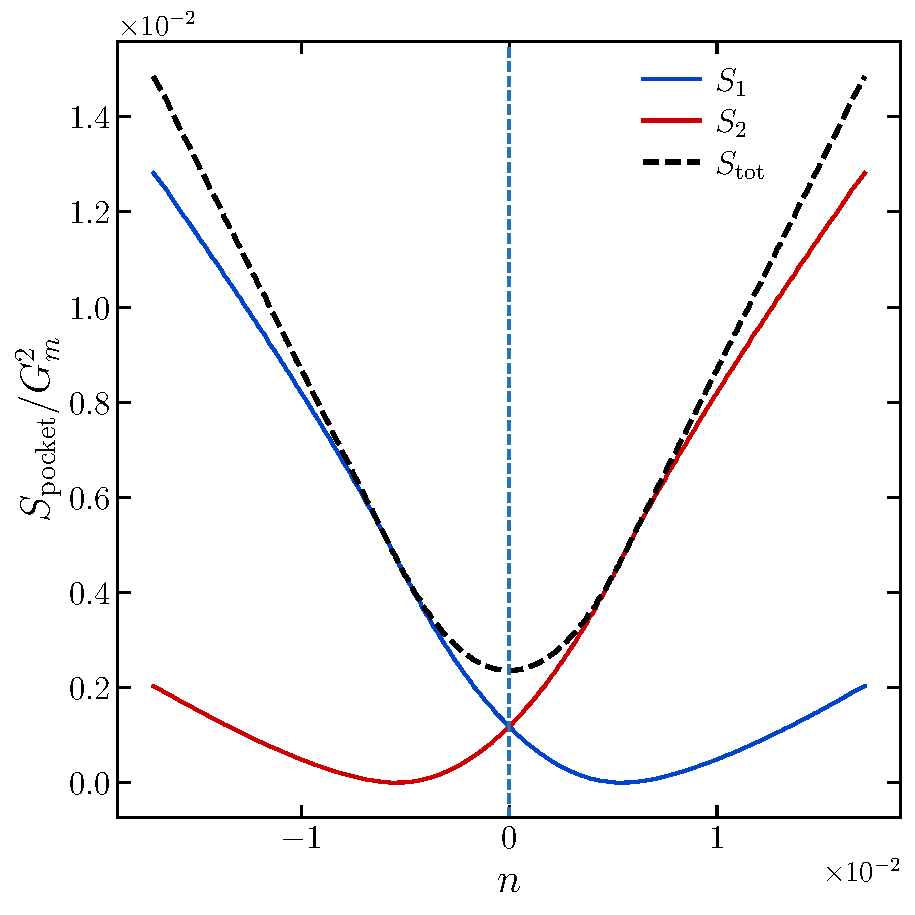
\includegraphics[width=0.40\textwidth]{fig/10/n_vs_area.pdf}
	\end{tabular}
	\caption{
		Pocket areas as a function of the normalized carrier density \(n\) in the two-pocket regime 
	}
	\label{fig10}
\end{figure}


\section{Appendix}

\subsection{Analytical expression of the wavefunctions at Dirac points}

In this appendix, we present the explicit analytical expressions of the two flat-band wavefunctions at the Dirac point in the truncated \(20\)-component basis. 

Since the unstrained BM Hamiltonian preserves \(C_{3z}\), the two degenerate states of Dirac points can be chosen as \(C_{3z}\) eigenstates. In a natural gauge, the two \(C_{3z}\) eigenvalues are \(e^{i2\pi/3}\) and \(1\). Since an overall gauge transformation changes these eigenvalues by a common phase while leaving physical quantities unchanged, we use the symmetric gauge \(e^{i\pi/3}\) and \(e^{-i\pi/3}\).

The \(C_{3z}\) symmetry is represented in this basis as \(C_{3z}^{(20)}=P_{C_3}\otimes D_{C_3}\), where \(P_{C_3}\) permutes the momentum points connected by threefold rotation and \(D_{C_3}\) acts on the two-component sublattice. We choose it as \(D_{C_3} = \exp\p{i\frac{\pi}{3}\sigma_z}\). The two eigenstates of Dirac points need to satisfy
\begin{align}
	C_{3z}^{(20)}\ket{\phi_n}
	=
	\lambda_n \ket{\phi_n},
	\qquad
	\lambda_1=e^{i\pi/3},
	\quad
	\lambda_2=e^{-i\pi/3}.
\end{align}
Together with the Schr\"odinger equation at Dirac points
\begin{align}
	H^{\p{20}}(\bm{K})\ket{\phi_n}=E_D\ket{\phi_n}, \qquad E_D = 0,
\end{align}
the symmetry condition fixes all components of the two eigenstates up to an overall normalization. 

\begin{align}
	\ket{\phi_1}
	=
	\mathcal{N}
	\begin{pmatrix}
		\phi_{1(1 \sim 4)} \\
		\phi_{1(5 \sim 6)} \\
		\phi_{1(7 \sim 8)} \\
		\phi_{1(9 \sim 10)}
	\end{pmatrix},
	\qquad
	\ket{\phi_2}
	=
	\mathcal{N}
	\begin{pmatrix}
		\phi_{2(1 \sim 4)} \\
		\phi_{2(5 \sim 6)} \\
		\phi_{2(7 \sim 8)} \\
		\phi_{2(9 \sim 10)}
	\end{pmatrix},
\end{align}
where each block is written as a row vector followed by a transpose. Choosing \(\phi_{12}^{A}=w_0\) for \(\ket{\phi_1}\) and \(\phi_{22}^{A}=w_1\) for \(\ket{\phi_2}\), we obtain the two wavefunctions. For \(\ket{\phi_1}\), we have
\begin{align}
	\begin{split}
		\phi_{1(1 \sim 4)}
	&=
	\begin{pmatrix}
		0 &
		i \p{\dfrac{w_{0}^{2}}{v_F \hbar \bv{\bm{q}_1}} - v_F \hbar \bv{\bm{q}_1}} &
		w_0 &
		- w_1 &
		e^{-i \frac{2\pi}{3}} w_0 &
		- w_1 &
		e^{i \frac{2\pi}{3}} w_0 &
		- w_1
	\end{pmatrix}^{T},
	\\[0.5em]
	\phi_{1(5 \sim 6)}
	&=
	\begin{pmatrix}
		- i \dfrac{w_0 w_1}{v_F \hbar \bv{\bm{q}_1}} &
		\dfrac{1}{\sqrt{3} v_F \hbar \bv{\bm{q}_1}}
		\p{- e^{i \frac{2\pi}{3}} w_{0}^{2} + e^{-i \frac{2\pi}{3}} w_{1}^{2}} &
		i e^{i \frac{\pi}{3}} \dfrac{w_0 w_1}{v_F \hbar \bv{\bm{q}_1}} &
		\dfrac{1}{\sqrt{3} v_F \hbar \bv{\bm{q}_1}}
		\p{e^{-i \frac{2\pi}{3}} w_{0}^{2} - e^{i \frac{2\pi}{3}} w_{1}^{2}}
	\end{pmatrix}^{T},
	\\[0.5em]
	\phi_{1(7 \sim 8)}
	&=
	\begin{pmatrix}
		- i e^{-i \frac{2\pi}{3}} \dfrac{w_0 w_1}{v_F \hbar \bv{\bm{q}_1}} &
		\dfrac{1}{\sqrt{3} v_F \hbar \bv{\bm{q}_1}}
		\p{- e^{i \frac{2\pi}{3}} w_{0}^{2} + e^{-i \frac{2\pi}{3}} w_{1}^{2}} &
		i e^{-i \frac{\pi}{3}} \dfrac{w_0 w_1}{v_F \hbar \bv{\bm{q}_1}} &
		\dfrac{1}{\sqrt{3} v_F \hbar \bv{\bm{q}_1}}
		\p{e^{-i \frac{2\pi}{3}} w_{0}^{2} - e^{i \frac{2\pi}{3}} w_{1}^{2}}
	\end{pmatrix}^{T},
	\\[0.5em]
	\phi_{1(9 \sim 10)}
	&=
	\begin{pmatrix}
		- i e^{i \frac{2\pi}{3}} \dfrac{w_0 w_1}{v_F \hbar \bv{\bm{q}_1}} &
		\dfrac{1}{\sqrt{3} v_F \hbar \bv{\bm{q}_1}}
		\p{- e^{i \frac{2\pi}{3}} w_{0}^{2} + e^{-i \frac{2\pi}{3}} w_{1}^{2}} &
		- i \dfrac{w_0 w_1}{v_F \hbar \bv{\bm{q}_1}} &
		\dfrac{1}{\sqrt{3} v_F \hbar \bv{\bm{q}_1}}
		\p{e^{-i \frac{2\pi}{3}} w_{0}^{2} - e^{i \frac{2\pi}{3}} w_{1}^{2}}
	\end{pmatrix}^{T}.
	\end{split}
\end{align}

For \(\ket{\phi_2}\), we obtain
\begin{align}
	\begin{split}
		\phi_{2(1 \sim 4)}
	&=
	\begin{pmatrix}
		i \p{\dfrac{w_{0}^{2}}{v_F \hbar \bv{\bm{q}_1}} - v_F \hbar \bv{\bm{q}_1}} &
		0 &
		w_1 &
		- w_0 &
		w_1 &
		- e^{i \frac{2\pi}{3}} w_0 &
		w_1 &
		- e^{- i \frac{2\pi}{3}} w_0
	\end{pmatrix}^{T},
	\\[0.5em]
	\phi_{2(5 \sim 6)}
	&=
	\begin{pmatrix}
		\dfrac{1}{\sqrt{3} v_F \hbar \bv{\bm{q}_1}}
		\p{e^{-i \frac{2\pi}{3}} w_{0}^{2} - e^{i \frac{2\pi}{3}} w_{1}^{2}} &
		- i \dfrac{w_0 w_1}{v_F \hbar \bv{\bm{q}_1}} &
		\dfrac{1}{\sqrt{3} v_F \hbar \bv{\bm{q}_1}}
		\p{- e^{i \frac{2\pi}{3}} w_{0}^{2} + e^{- i \frac{2\pi}{3}} w_{1}^{2}} &
		i e^{-i \frac{\pi}{3}} \dfrac{w_0 w_1}{v_F \hbar \bv{\bm{q}_1}}
	\end{pmatrix}^{T},
	\\[0.5em]
	\phi_{2(7 \sim 8)}
	&=
	\begin{pmatrix}
		\dfrac{1}{\sqrt{3} v_F \hbar \bv{\bm{q}_1}}
		\p{e^{-i \frac{2\pi}{3}} w_{0}^{2} - e^{i \frac{2\pi}{3}} w_{1}^{2}} &
		- i e^{i \frac{2\pi}{3}} \dfrac{w_0 w_1}{v_F \hbar \bv{\bm{q}_1}} &
		\dfrac{1}{\sqrt{3} v_F \hbar \bv{\bm{q}_1}}
		\p{- e^{i \frac{2\pi}{3}} w_{0}^{2} + e^{- i \frac{2\pi}{3}} w_{1}^{2}} &
		i e^{i \frac{\pi}{3}} \dfrac{w_0 w_1}{v_F \hbar \bv{\bm{q}_1}}
	\end{pmatrix}^{T},
	\\[0.5em]
	\phi_{2(9 \sim 10)}
	&=
	\begin{pmatrix}
		\dfrac{1}{\sqrt{3} v_F \hbar \bv{\bm{q}_1}}
		\p{e^{-i \frac{2\pi}{3}} w_{0}^{2} - e^{i \frac{2\pi}{3}} w_{1}^{2}} &
		- i e^{- i \frac{2\pi}{3}} \dfrac{w_0 w_1}{v_F \hbar \bv{\bm{q}_1}} &
		\dfrac{1}{\sqrt{3} v_F \hbar \bv{\bm{q}_1}}
		\p{- e^{i \frac{2\pi}{3}} w_{0}^{2} + e^{- i \frac{2\pi}{3}} w_{1}^{2}} &
		- i \dfrac{w_0 w_1}{v_F \hbar \bv{\bm{q}_1}}
	\end{pmatrix}^{T}.
	\end{split}
\end{align}

The common normalization coefficient of \(\ket{\phi_1}\) and \(\ket{\phi_2}\) is
\begin{align}
	\mathcal{N}
	=
	\p{
		w^2_{0} + 3 w_{1}^{2} + v_{F}^{2} \hbar ^2 \bv{\bm{q}_{1}}^2
		+ \frac{3 w_{0}^4 + 8 w_{0}^2 w_{1}^2 + 2 w_{1}^4}{v_{F}^{2} \hbar^2 \bv{\bm{q}}_{1}^{2}}
	}^{-1/2}.
\end{align}


\subsection{Condition for \(C_{2x}\) symmetry under heterostrain}

In this appendix, we derive the conditions for \(C_{2x}\) symmetry to be preserved in the TBG under heterostrain.

The representation matrix of \(C_{2x}\) is \(\tau_{x} \bigotimes \sigma_{x} \), which is 
\begin{align}
	U_{C_{2x}} = \tau_{x} \otimes \sigma_{x} = \begin{pmatrix}
		0 & \sigma_{x} \\
		\sigma_{x} & 0
	\end{pmatrix}.	
\end{align}
The Hamiltonian should satisfy \(H(C_{2x} \bm{k}) = U_{C_{2x}} H(\bm{k}) U_{C_{2x}}^{\dagger}\). Substituting the Hamiltonian into the commutation relation, we have \(H_{t/b}\p{C_{2x}\bm{k}} = \sigma_{x} H_{b/t}\p{\bm{k}} \sigma_{x}\). To satisfy the \(C_{2x}\) symmetry, we need to rewrite the Hamiltonian as the symmetric form where the origin set as \(\bm{\Gamma}_{m}\) from \(\bm{K}_{t}\) point. The Hamiltonian of two layers can be written as
\begin{align}
	\begin{split}
		H_{t}\p{\bm{k}} & = v_{F} \hbar \bb{\bm{k} - \bm{Q}_{t}} \cdot \bm{\sigma} + \alpha \vph \mathbb{I} + v_{F} \gamma \bm{A} \cdot \bm{\sigma} \\
		H_{b}\p{\bm{k}} & = v_{F} \hbar \bb{\bm{k} - \bm{Q}_{b}} \cdot \bm{\sigma} - \alpha \vph \mathbb{I} - v_{F} \gamma \bm{A} \cdot \bm{\sigma},
	\end{split}
\end{align}
where geometry asks 
\begin{align}
		\bm{Q}_{t}  = \bm{K}_{t} - \bm{\Gamma}_{m}, \quad \bm{Q}_{b} = \bm{K}_{b} - \bm{\Gamma}_{m}.
\end{align}
For the scalar term, the commutation relation requires
\begin{align}
	- \alpha \vph \mathbb{I} = \sigma_{x} \alpha \vph \mathbb{I} \sigma_{x},
\end{align}
which leads to 
\begin{align}
	\vph = 0 \Leftrightarrow \epsilon_{1} = - \epsilon_{2} \Leftrightarrow \nu = 1.
\end{align}
And the vector term 
\begin{align}
	- v_{F} \gamma \p{A_{x} \bm{\sigma}_{x} + A_{y} \bm{\sigma}_{y}} = v_{F} \gamma \p{A_{x} \bm{\sigma}_{x} - A_{y} \bm{\sigma}_{y}},
\end{align}
and we get
\begin{align}
	A_{x} = 0 \Leftrightarrow \cos{2 \phi} = 0 \Leftrightarrow \phi = \p{\frac{n}{2}+ \frac{1}{4}} \pi,
\end{align}
which means the direction of principle axes of strain is along the \(k_y\) axis. Also, the momentum term is naturally satisfied the commutation relation.

The corresponding critical strain magnitude \(\epsilon\) can in principle be determined by solving
\begin{align}
	E(\bm{q}_1/2)=0,
\end{align}
but it is difficult to solve analytically.

\subsection{Relation between carrier density and pocket area in a two-Dirac-cone model}

In this appendix, we derive the relation between the carrier density and the Fermi-surface pocket area in a simplified two-Dirac-cone model. 

For the carriers' density \(n\), we have its definition as the integral of the Fermi-Dirac distribution \(f\p{E}\) of the two center bands over the Brillouin zone (BZ)
\begin{align}
	n\p{E_{F}} = \frac{1}{\p{2 \pi}^2} \int_{\mr{BZ}} d^2 \bm{k} \bb{f\p{E_{top}} + f\p{E_{bot}} - 1}.
\end{align}
Due to the particle-hole symmetry, the energy of charge neutrality point is zero. At \(T = 0 K\), the density of carriers is 
\begin{align}
	\begin{split}
		n\p{E_F} & = \frac{1}{\p{2 \pi}^2} \int_{\mr{BZ}} d^2 \bm{k} \bb{\Theta \p{E_{F} - E_{top} \p{\bm{k}}} + \Theta \p{E_{F} - E_{bot} \p{\bm{k}}} - 1} \\
		& = \frac{1}{N_{\bm{k}}} \sum_{\bm{k}} \bb{\Theta \p{E_{F} - E_{top}\p{\bm{k}}} + \Theta \p{E_{F} - E_{bot} \p{\bm{k}}} - 1},
	\end{split}
\end{align}
where \(N_{\bm{k}}\) is the total \(\bm{k}\) point in the reciprocal primitive cell.

For two perfect Dirac cones which its energies shifted by \(E_0\) and \(-E_0\). With the Fermi level \(-E_0 < E_F < E_0\), the carrier density \(n\) actually is the difference area of electron pocket and hole pocket \(S_{e} - S_{h}\). We can rewrite the definition as \(n = 1/N_{\bm{k}} \sum_{\bm{k}} I \p{\bm{k}}\) and \(I \p{\bm{k}} = \Theta \p{E_{F} - E_{top}\p{\bm{k}}} + \Theta\p{E_{F} - E_{bot}\p{\bm{k}}} - 1\). With \(\Theta\p{E_F - E_{top} \p{\bm{k}}} + \Theta \p{E_{top} \p{\bm{k}} - E_{F}} = 1\), \(I \p{\bm{k}}\) is 
\begin{align}
	\begin{split}
		I \p{\bm{k}} & = \Theta \p{E_F - E_{top}} + \Theta \p{E_F - E_{bot}} - \Theta \p{E_{F} - E_{top}} - \Theta \p{E_{top} - E_{F}} \\
		& = \Theta \p{E_F - E_{bot}} - \Theta \p{E_{top} - E_{F}} \\
		& = S_{e} - S_{h}.
	\end{split}
\end{align}
It means the bottom band corresponding to the higher Dirac point with \(+ E_0\) gives the hole pocket and the top band corresponding to the lower Dirac point with \(- E_0\) gives the electron pocket. For perfect Dirac cones with the energy dispersion of \(E_{t}\p{\bm{p}} =  - E_0 + v_F |\bm{p}|\) and \(E_{b}\p{\bm{p}^\prime} = E_0 + v_F |\bm{p}^\prime|\), The electron pocket from the top band with the Fermi level \(E_F\) has the area of \(S_{\mr{e}} = \pi \p{\frac{E_0 + E_F}{\hbar v_F}}^2\) and the hole pocket from the bottom band has the area of \(S_{\mr{h}} = \pi \p{\frac{E_0 - E_F}{\hbar v_F}}^2\). The total area of the two pockets is \(S_{\mr{e}} + S_{\mr{h}}\)
\begin{align}
	S_{\mr{tot}} = \pi \p{\frac{E_0 + E_F}{\hbar v_F}}^2 + \pi \p{\frac{E_0 - E_F}{\hbar v_F}}^2 = \frac{2 \pi}{\hbar^2  v_F^2} \p{E_0^2 + E_F^2}.
\end{align}
The carrier density is \(n = S_{\mr{e}} - S_{\mr{h}} = 4 \pi \frac{E_F E_0}{\hbar^2 v_F^2}\). Thus, \(E_F = \frac{n \hbar^2 v_F^2}{4 \pi E_0}\). Substituting it into the total area of two pockets, we have the relation of carrier density \(n\) with the total pocket area \(S_{\mr{pocket}}\) 
\begin{align}
	S_{\mr{pocket}} = \frac{2 \pi E_0^2}{\hbar^2 v_F^2}  + \frac{n^2 \hbar^2 v_F^2}{8 \pi E_0^2}.
\end{align}
For the hole/electron pocket, the relation of area with carrier density is 
\begin{align}
	S_{\mr{e/h}} = \pi \p{ \frac{n^2 \hbar^2 v^{2}_{F}}{16 \pi^2 E^2_0} \pm \frac{n}{2}+ \frac{E_0^2}{\hbar^2 v_F^2}}.
\end{align}

When we consider a large energy regime like \(E_F > E_{0}\), the hole pocket changes into an electron pocket, both of which are a large electron pocket and a small electron pocket. The carrier density is \(n = S_{e;l} + S_{e;s}\). Thus, the area of the new smaller electron pocket is 
\begin{align}
	S_{e, s} = \frac{n}{2} - \sqrt{\frac{2 \pi E^2_0}{\hbar^2 v^2_{F}} n - \p{\frac{2 \pi E^2_0}{\hbar^2 v^2_{F}}}^2},
\end{align}
where \(n = \frac{2 \pi }{\hbar^2 v^2_{F}} \p{E^2_{F} + E^2_{0}}, \, E_{F} = \sqrt{\frac{\hbar^2 v^2_{F}}{2 \pi} n - E^2_0}\) and \(n = \frac{2 \pi E^2_0}{\hbar^2 v^2_{F}}\) is the zero point for both relations in the two energy regimes.  

For the Dirac cone under heterostrain, we need to substitute the Fermi velocity \(v_F\) with the renormalized Fermi velocity \(v^{*}\).

\end{document}
